%%%%%%%%%%%%%%%%%%%%%%%%%%%%%%%%%%%%%%%%%%%%%%%%%%%%%%%%%%%%%%%%%%%%%%
%% Converted from IEEEtran (main.tex) to the Springer Nature sn-jnl   %%
%% template (sn-article.tex). Content is preserved from the original %%
%% manuscript; only formatting/structure was adapted to sn-jnl.      %%
%%%%%%%%%%%%%%%%%%%%%%%%%%%%%%%%%%%%%%%%%%%%%%%%%%%%%%%%%%%%%%%%%%%%%%

\documentclass[pdflatex,sn-mathphys-num]{sn-jnl}% Math and Physical Sciences Numbered Reference Style

%%%% Standard Packages
%%<additional latex packages if required can be included here>

\usepackage{graphicx}%
\usepackage{multirow}%
\usepackage{amsmath,amssymb,amsfonts}%
\usepackage{amsthm}%
\usepackage{pgfplots}%
\usepackage{mathrsfs}%
\usepackage[title]{appendix}%
\usepackage{xcolor}%
\usepackage{textcomp}%
\usepackage{manyfoot}%
\usepackage{booktabs}%
\usepackage{algorithm}%
\usepackage{algorithmicx}%
\usepackage{algpseudocode}%
\usepackage{listings}%
%% Additional packages required by the original manuscript (main.tex)
\usepackage{url}%
\usepackage{array}%
\usepackage{adjustbox}%
\usepackage{tabularx}%
%%%%

\graphicspath{{figs/}}
\pgfplotsset{compat=1.18}

%% as per the requirement new theorem styles can be included as shown below
\theoremstyle{thmstyleone}%
\newtheorem{theorem}{Theorem}%  meant for continuous numbers
\newtheorem{proposition}[theorem]{Proposition}%

\theoremstyle{thmstyletwo}%
\newtheorem{example}{Example}%
\newtheorem{remark}{Remark}%

\theoremstyle{thmstylethree}%
\newtheorem{definition}{Definition}%

\raggedbottom

\begin{document}

\title[Building the Cities of Tomorrow]{Building the Cities of Tomorrow: Technology, Infrastructure, and Sustainability}

%%=============================================================%%
%% GivenName	-> \fnm{Joergen W.}
%% Particle	-> \spfx{van der} -> surname prefix
%% FamilyName	-> \sur{Ploeg}
%% Suffix	-> \sfx{IV}
%%=============================================================%%

\author[1]{\fnm{Jaishnu Sree} \sur{Biradha}}

\author[1]{\fnm{Derrick} \sur{Richard}}

\author*[1]{\fnm{Suseela} \sur{Sellamuthu}}\email{suseela.s@vit.ac.in}

\author[1]{\fnm{Bhavadharini} \sur{R. M.}}

\author[1]{\fnm{Krithiga} \sur{R.}}

\affil*[1]{\orgdiv{School of Computer Science and Engineering (SCOPE)}, \orgname{Vellore Institute of Technology}, \orgaddress{\city{Chennai}, \state{Tamil Nadu}, \country{India}}}

\abstract{Smart cities bring together networked data systems and new approaches to governance and operations, with the aim of improving residents' quality of life, lowering environmental impact, and supporting economic growth. This review looks at the technologies behind smart urban development, mainly the Internet of Things (IoT), artificial intelligence (AI), big data analytics, and renewable energy. It then turns to the infrastructure required to use these technologies across a whole city, including intelligent transport, energy-efficient buildings, waste-management systems, and dependable digital connectivity. Using examples from Dubai, Barcelona, Singapore, New York City, and other metropolitan areas, the review pulls out practical lessons from what these cities have actually done. It also covers the partnerships, multilateral initiatives, and interoperability standards that help smart city programs grow and link up across borders. The paper closes with a framework for future development that stresses ongoing cooperation among stakeholders, clear governance and regulation, and long-term planning for the urban challenges still to come.}

\keywords{Artificial Intelligence (AI), 5G Wireless Networks, Smart Cities, Digital Infrastructure, Intelligent Transportation Systems (ITS), Global Governance, Internet of Things (IoT), Sustainable Development Goals (SDGs)}

\maketitle

\section{Introduction}
\textbf{Smart cities} have become a leading model of urban living over the past few decades, largely thanks to progress in digital technology. At their heart is \textbf{information and communication technology (ICT)}, which cities rely on to plan and run essential services more efficiently and to make daily life better for residents. Typical applications include \textbf{digital healthcare}, \textbf{intelligent transport}, technology-enabled retail, \textbf{connected homes}, education, and joined-up energy and transportation infrastructure, as shown in Fig.~\ref{fig:services}.
\begin{figure}[ht]
\centering
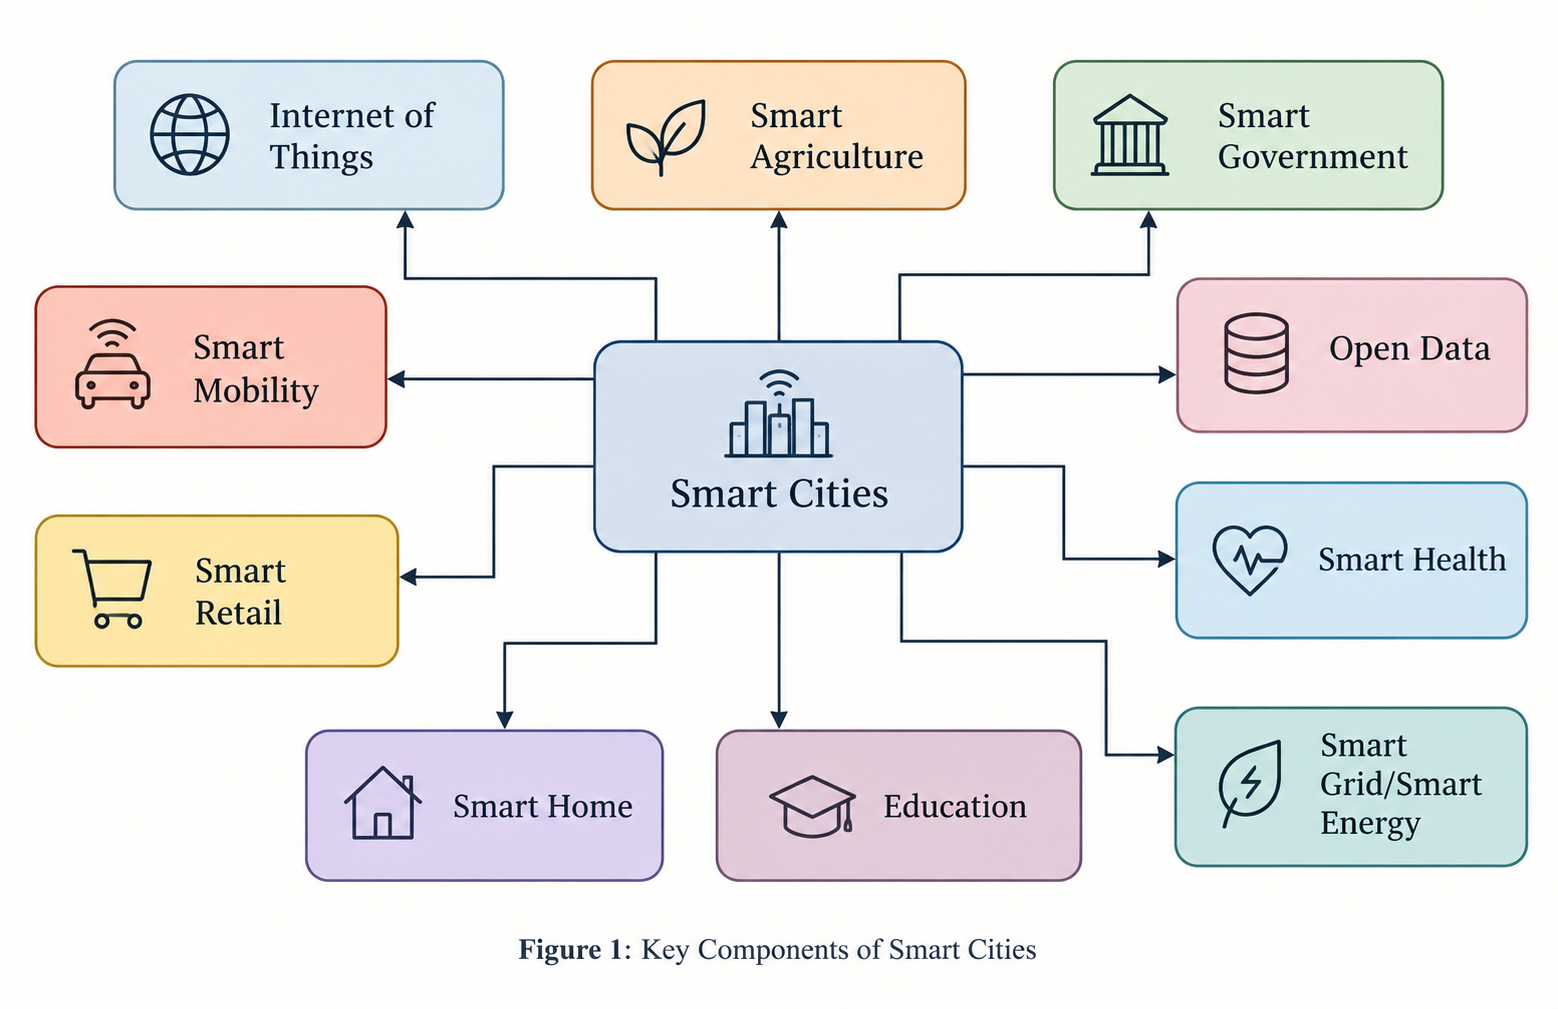
\includegraphics[width=\linewidth]{image-001.png}
\caption{Smart Cities Services}
\label{fig:services}
\end{figure}

Building digital systems into a city's infrastructure helps cities use fewer resources, make better administrative decisions, and get more residents involved. Table~\ref{tab:urban_projections} summarizes the demographic and environmental trends of global urbanization, and they make the case for action clear: cities use between 66\% and 75\% of the world's primary energy and produce over 70\% of global greenhouse gas emissions, even though they take up only 2\% to 3\% of the Earth's land \cite{r124}. With global urban population projected to expand from 56.2\% to 68.4\% by 2050---adding approximately 2.5 billion new residents predominantly across Asia and Africa---\textbf{data-driven municipal ecosystems} are indispensable to avert severe resource strain \cite{r1,r5}. Fig.~\ref{fig:framework} illustrates a smart urban environment as an integrated network of \textbf{IoT-enabled devices}, \textbf{sensing units}, and \textbf{cloud computing infrastructure}, collectively gathering, transmitting, and analyzing data continuously in real time.

\begin{table}[!t]
\caption{Global Urban Demographics, Resource Footprint, and 2050 Projections [Source: United Nations DESA \cite{r124} and UN-Habitat]}
\label{tab:urban_projections}
\centering
\scriptsize
\setlength{\tabcolsep}{3pt}
\renewcommand{\arraystretch}{1.2}
\renewcommand{\tabularxcolumn}[1]{m{#1}}
\begin{tabularx}{\linewidth}{|
>{\raggedright\arraybackslash}m{0.32\linewidth}|
>{\centering\arraybackslash}m{0.20\linewidth}|
>{\centering\arraybackslash}m{0.20\linewidth}|
>{\raggedright\arraybackslash}X|}
\hline
\textbf{Indicator / Metric} & \textbf{Historical (2020)} & \textbf{Projected (2050)} & \textbf{Key Impact / Significance} \\
\hline
Global Urban Population & 4.38 Billion & 6.68 Billion & +2.3--2.5B net urban influx \\
\hline
Share of World Population & 56.2\% & 68.4\% & $\sim$90\% growth concentrated in Asia \& Africa \\
\hline
Terrestrial Land Occupancy & $\sim$2.0\%--3.0\% & $\sim$3.5\% & Severe spatial concentration of resource demand \\
\hline
Global Primary Energy Use & 67\%--75\% & 75\%--80\% & Driven heavily by buildings, mobility, and industry \\
\hline
Global Energy-Related GHG & 71\%--76\% & 75\%--82\% & Primary battleground for international climate targets \\
\hline
Solid Waste Generation & 2.01 Bt/year & 3.40 Bt/year & +70\% expansion requiring IoT circular logistics \\
\hline
\end{tabularx}
\end{table}

\begin{figure}[ht]
\centering
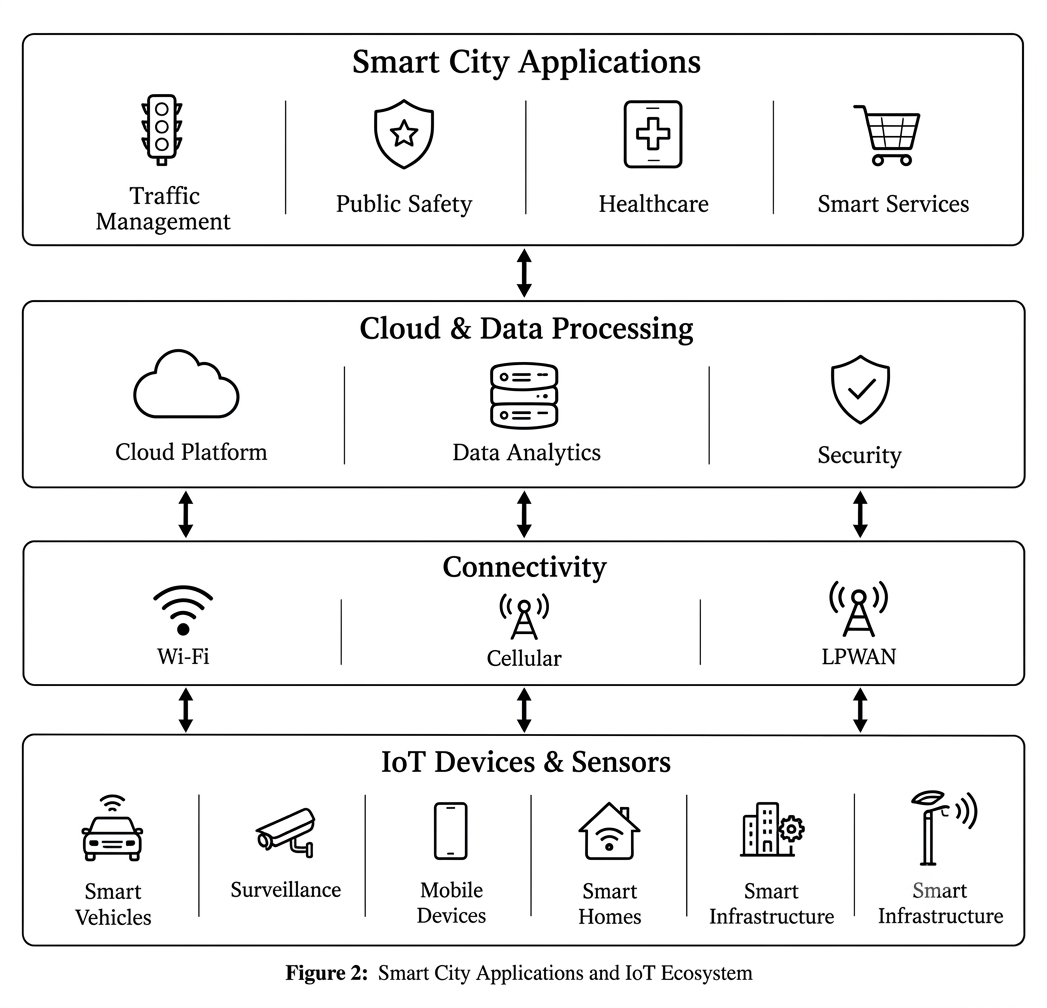
\includegraphics[width=\linewidth,height=0.5\textheight,keepaspectratio]{image-002.png}
\caption{Smart City Framework}
\label{fig:framework}
\end{figure}

This real-time information base allows city administrations to make better-informed decisions, whether in optimizing traffic flow, regulating energy distribution, or improving public safety \cite{r1}. \textbf{Road-monitoring systems}, for example, assess pavement and traffic conditions and adjust signal timing accordingly, reducing congestion and emissions \cite{r3}. \textbf{Smart grids} allocate electricity more efficiently, cutting waste and directing power to where it is most needed. Beyond raising operational efficiency, such technologies help cities meet sustainability targets that become more pressing as urban populations continue to grow \cite{r4}. Shao and Min catalog a broad range of sustainability measures relevant to smart city development \cite{r107}, while noting that multidimensional sustainability models remain largely confined to conceptual frameworks rather than operational practice. Singh \emph{et al.} take a broader historical view, tracing a decade of technological advances, architectural models, and platforms in smart city research \cite{r108}. Their survey of sensing technologies, communication layers, data management, and application domains gives the study of smart urban development a solid technical footing. It also points to \textbf{governance integration}, \textbf{citizen engagement}, \textbf{global interoperability}, and cross-case comparison as areas that still need more attention. Han and Kim similarly note a lasting gap between technology-focused research and the realities of urban environments, governance structures, infrastructure integration, and international benchmarking \cite{r7}.

Smart city research has grown quickly, but there are still open questions about how technology, infrastructure, and governance work together in different urban settings. This review looks at innovation, technology, and infrastructure in a global context, alongside governance, inclusion, international standards, and examples from Dubai, Singapore, Barcelona, and New York City. It links technological innovation to physical and virtual infrastructure, citizen participation, and sustainability goals, and it brings out unresolved issues around \textbf{data privacy}, \textbf{social equity}, and regulation.

As smart technologies become more widespread, collaboration and standardisation have become key to making them work. Cities use \textbf{international standards}, partnerships, and city networks to share practices, data, and resources, and to build the \textbf{interoperability} that connects individual cities across borders. Singapore, Barcelona, Dubai, and New York City illustrate this combination of urban innovation and international collaboration \cite{r8}. Yet data privacy, security, inclusion, and resilient policy frameworks have become harder to manage as these capabilities expand. The same technologies that improve efficiency also increase the volume of data that must be managed and make equitable access harder to ensure \cite{r9,r101}.

This review addresses policymakers, academics, and professionals working across the urban technology sector in developed as well as developing economies, with the aim of clarifying the progression of smart cities, the difficulties associated with their implementation, and the strategies required to create urban environments that are better connected, adaptable, and accessible to diverse populations. It further examines the integration of technological advancement, innovation, and physical infrastructure as mechanisms for reshaping urban living, while emphasizing the importance of cross-border collaboration in expanding these advantages among prominent metropolitan areas, including Dubai, Barcelona, Singapore, and New York City. \cite{r12,r13}.

\begin{figure}[ht]
\centering
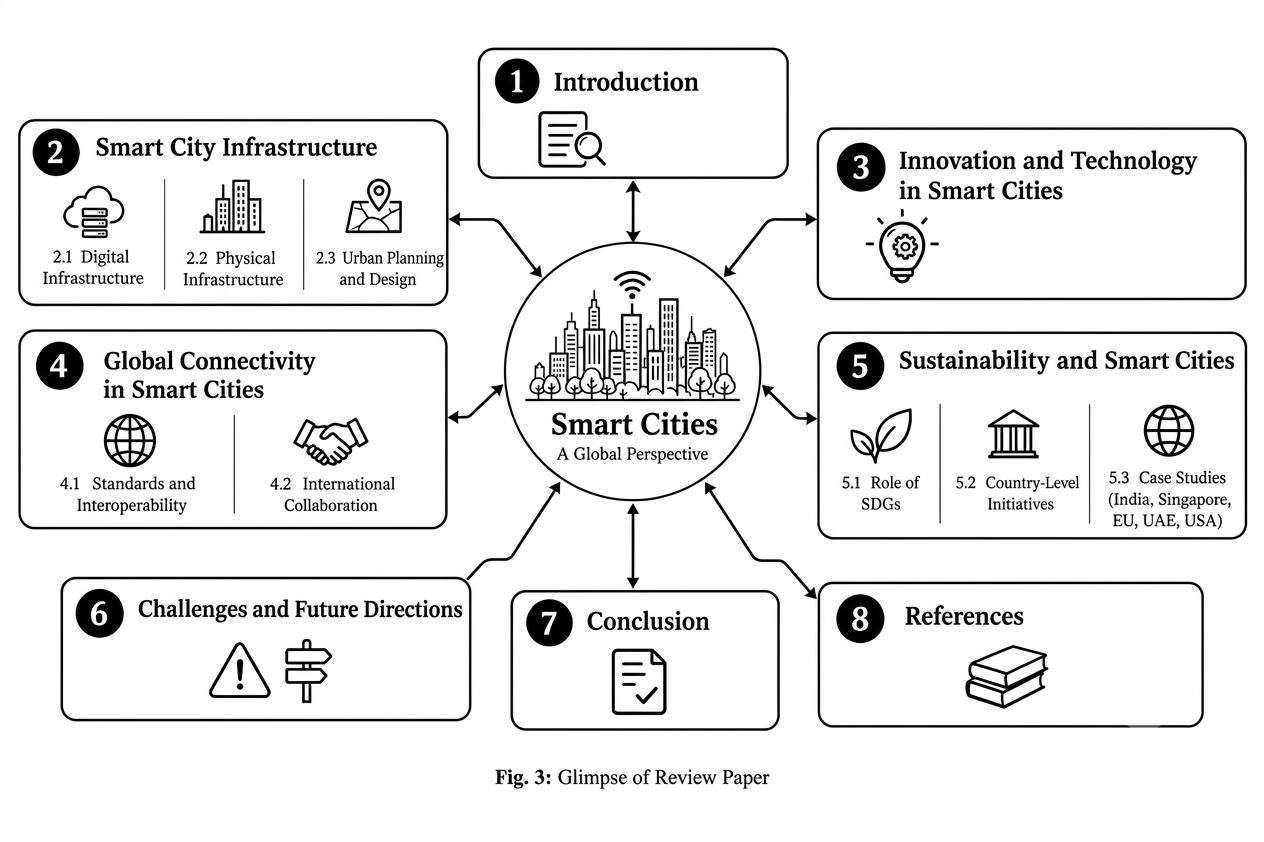
\includegraphics[width=\linewidth]{image-002(1).png}
\caption{Glimpse of Review Paper}
\label{fig:outline}
\end{figure}

The structure of the paper is illustrated in Fig.~\ref{fig:outline}. Section II focuses on the infrastructure that supports smart urban environments, while Section III reviews major innovations and technological developments. Section IV looks at how smart cities are connected with one another around the world. Section V examines the role the Sustainable Development Goals (SDGs) play in smart city development. Section VI sets out the main challenges in this area and suggests where future progress might come from. Finally, Section VII offers the concluding remarks.

\section{Smart City Infrastructure}
\noindent This part looks at digital infrastructure, physical infrastructure, and urban planning and design as the three pillars of smart city infrastructure.

As cities grow quickly, they are under more pressure to manage services effectively and responsibly, which puts infrastructure at the center of smart urban development. \textbf{Smart city infrastructure} brings existing municipal assets together with digital systems so that public services improve, resources go further, and communication gets stronger. This kind of integration supports technology-driven services that raise residents' well-being and help cities stay sustainable over the long run, though it only works when the different infrastructure components are well coordinated. As Fig.~\ref{fig:infrastructure} shows, this section sorts infrastructure requirements into three areas: \textbf{digital infrastructure}, \textbf{physical infrastructure}, and \textbf{urban planning and design}.

\begin{figure}[ht]
\centering
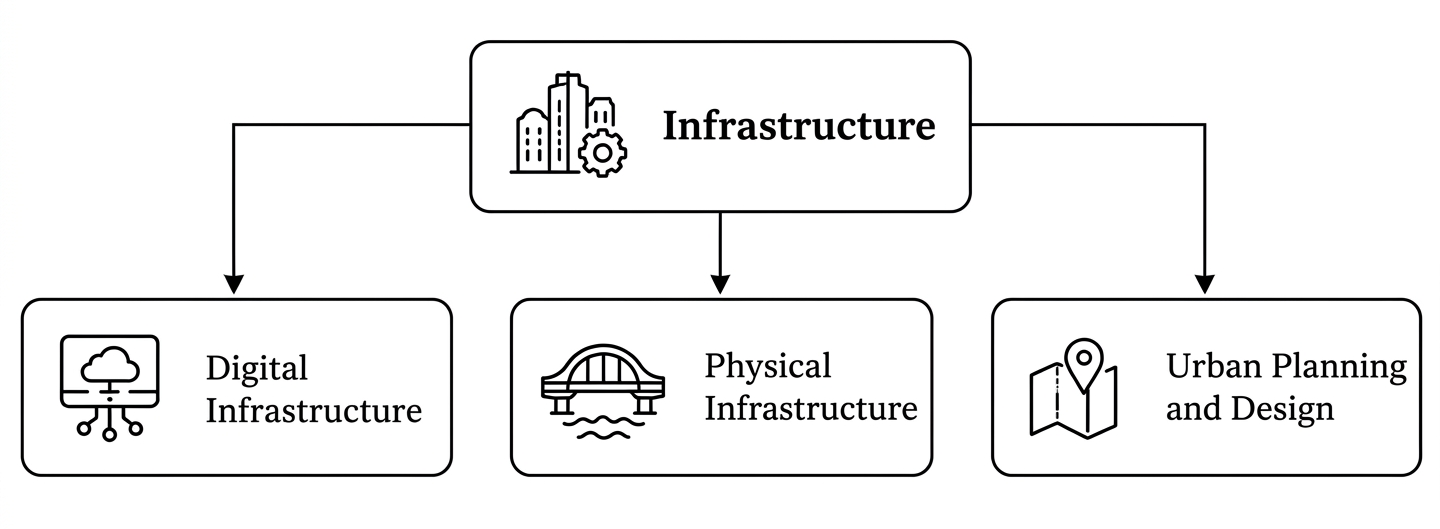
\includegraphics[width=\linewidth]{image-003.png}
\caption{Smart City Infrastructure}
\label{fig:infrastructure}
\end{figure}

\subsection{Technological Infrastructure Supporting Smart Urban Environments}
\noindent This part looks at how urban infrastructure has evolved over time and how digital infrastructure (ICT, sensors, cloud, and data centers) became the technological foundation of smart cities.

Urban infrastructure has changed a great deal over the centuries. Early settlements got by with simple systems for transport, water, and sanitation. The Industrial Revolution then brought railway networks, electric power grids, and telecommunications. Toward the end of the twentieth century, the internet and digital computing added yet another layer of capability. Today's cities link these established systems with intelligent technologies so they can keep up with the demands of modern urbanization.

Digital infrastructure forms the technological base for smart urban systems, since it ties municipal operations together and allows information to flow between them.As Fig.~\ref{fig:components} shows, it combines information and communication technologies (ICT), distributed sensors, cloud resources, and data centers to support coordinated administration and timely decisions. These components allow information to be collected, stored, analyzed, and transmitted across the city. The main elements are IoT sensors and devices, communication and networking layers, edge processing, cloud environments, and applications for smart city services.

\begin{figure}[ht]
\centering
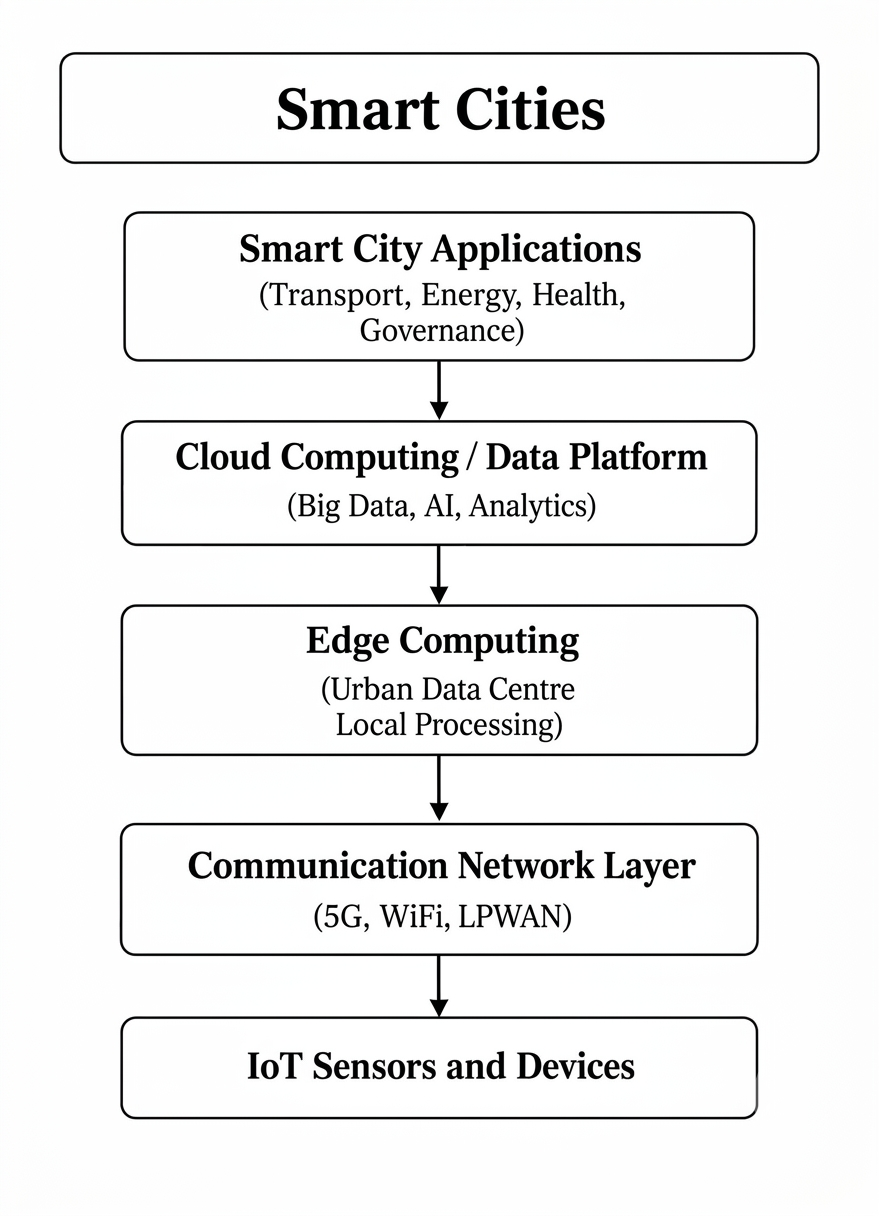
\includegraphics[width=0.72\linewidth,height=0.5\textheight,keepaspectratio]{image-004.png}
\caption{Components of Smart Cities}
\label{fig:components}
\end{figure}

Digital infrastructure allows smart cities to strengthen service delivery and operational effectiveness while extending connectivity to citizens. It underpins the latest generation of urban technologies aimed at improving city life, managing resources, and enhancing service quality, and is turning cities into platforms enabling urban environments to support continuous observation, evidence-based decisions, and adaptive responses to changing conditions. Investment in this infrastructure continues to grow, and studies have documented the substantial economic returns generated by smart city investment \cite{r102}.

\subsubsection{Key Elements of Digital Infrastructure}
As Fig.~\ref{fig:components} shows, these elements form a coordinated environment for collecting and exchanging information. Sensors in IoT systems observe the physical environment, and urban data centers store and analyze the resulting data. Cloud infrastructure adds computing capacity that can grow or shrink with demand. These components depend on shared technologies, communication protocols, and technical standards so they can work together and exchange information. The digital foundation that results supports a growing range of urban applications and services.

IoT sensors keep track of urban conditions such as temperature, humidity, air pollution, traffic, and electricity use. Spread across a city, they produce a steady stream of data that helps authorities oversee and adjust municipal operations. An intelligent traffic signal, for example, can use sensor data to change its timing as vehicle volumes shift, which cuts congestion and emissions. IoT applications in mobility, energy, and asset management can also bring economic benefits to municipalities \cite{r15}.

Getting these benefits takes coordinated decisions about where to place sensors, how to transmit and process the data, and how to connect new systems with existing urban infrastructure. Cities also need strong safeguards for cybersecurity and personal privacy, along with clear ethical rules. When these needs are handled together, IoT investments can deliver more value and help cities run more effectively, recover from disruptions, and work toward sustainability goals \cite{r15}.

IoT technologies make it possible to automate services and make them interoperable across many city functions. To cope with the data these devices generate, data centers supply computing, storage, and networking capacity. Modern facilities rely on virtualization and container-based architectures to make better use of hardware, run more efficiently, and keep services available. Data centers are therefore a core part of smart city infrastructure, providing the scalable processing and storage needed to manage and make sense of urban data \cite{r16}.

Cloud computing offers processing and storage over the internet, so municipalities can run smart applications without spending heavily on on-premises hardware. These platforms handle data storage, large-scale analysis, and machine learning, all of which underpin many intelligent urban applications. Data from multiple sources can be pooled in the cloud and analyzed to produce insights for municipal decision-making. The growing use of cloud infrastructure for storage, analytics, and machine learning also shows how cloud computing and IoT are coming together in modern cities \cite{r10}.

Urban data platforms pull together information from sensors, social media, public datasets, and other digital sources. By offering a shared space for exchanging data, they help municipal departments and other stakeholders coordinate their work. Analytical and visualization tools help authorities make sense of complex datasets and turn the findings into policy. For example, bringing road conditions, weather, and public transport data together in one platform can support more efficient management of urban mobility.

\subsubsection{Implications of Digital Infrastructure}
\noindent This part looks at smart mobility, public safety, smart energy management, smart grids, and broadband connectivity (satellite, wireless, and fiber) as key application domains of digital infrastructure.

Digital infrastructure is reshaping urban transport by changing how mobility networks are organized and run. Research on ICT-enabled service frameworks for smart mobility shows that these systems can support sustainability, make transport more efficient, and improve quality of life in cities \cite{r107,r15}. Pairing IoT sensing with data analytics lets cities respond to traffic more quickly, which cuts congestion and journey times. Syncing public transport schedules and service availability in real time can also make transit networks more dependable. Smart parking is a good example: connected sensors report which spaces are free, so drivers find a spot sooner and spend less time circling, which lowers emissions. Intelligent traffic management can further improve operations and road safety while easing congestion, and this brings economic benefits to urban areas \cite{r12}.

Digital infrastructure also supports public safety through surveillance and data-informed emergency response. Facial recognition and video analysis let authorities keep an eye on incidents as they unfold. IoT devices such as acoustic gunshot detectors can warn law enforcement of threats early, before a situation gets worse. Adaptive street lighting changes its brightness when it detects activity, which may help discourage crime \cite{r13,r17}. New York City's Domain Awareness System shows how this works at scale: it pulls in data from more than 9,000 cameras and gives law enforcement real-time information. The system helps officers make faster, better-informed decisions during high-priority incidents and has contributed to crime-reduction efforts \cite{r14,r18}.

Digital infrastructure supports smart energy management by tracking and adjusting consumption across buildings and municipal facilities. Research on IoT-enabled energy systems for buildings and urban infrastructure shows that these technologies collect and analyze data, so energy use can be measured, controlled, and optimized. Better energy management can reduce environmental impact while also improving day-to-day efficiency and long-term sustainability \cite{r108,r19}.

Smart grids use IoT sensors to watch electricity supply and demand and to cut energy losses. Smart meters give users immediate information about how much they are consuming, which nudges them toward more efficient use. Metering data also lets municipalities and utilities set dynamic tariffs that move energy-intensive activity to times of lower demand. Sensing and communication across the grid can further reduce losses during transmission and distribution, which matters because many smart city services need large amounts of energy \cite{r98}.

Satellite broadband brings internet access to remote and rural areas that terrestrial networks do not reach. It can reach speeds of up to 100 Mbps, but latency is usually higher because signals have to travel to and from orbit. Even so, space-based services are growing as a complement to terrestrial networks and are helping close connectivity gaps in underserved areas \cite{r20,r21}.

Wireless broadband, including fourth-generation LTE and emerging 5G networks, offers high-speed connectivity without fixed cabling. Wireless networks tend to be more flexible and easier to scale than wired systems. They matter most for mobile users and for places where wired infrastructure is technically difficult or too costly to roll out. As 5G spreads and smart city systems demand more network capacity, wireless broadband will only become more important \cite{r22}.

Fast internet forms the communication layer for smart buildings and homes, linking IoT devices, security systems, and appliances. With reliable connectivity, occupants can monitor and control energy use, security, and indoor conditions from a distance. Stable, high-speed broadband is therefore essential for the remote monitoring and control that connected homes and intelligent buildings rely on \cite{r23}.

Fast internet is just as essential for intelligent transport, tying together autonomous vehicles, street lighting, and real-time transit management systems. Constant communication between these assets can smooth vehicle movement and reduce congestion. Since human error causes a large share of road accidents, combining broadband connectivity with automated and connected driving offers a real chance to make roads safer \cite{r24}.

Fast internet also makes it easier to deliver government services online, which increases transparency and lowers administrative costs; citizens can pay bills and handle civic business from home instead of visiting an office. Countries with more developed broadband infrastructure tend to score higher on the e-government development index (EGDI), reflecting easier access to electronic government services \cite{r25}.

Reliable broadband is now a basic requirement for online learning, giving students and educators access to digital resources, virtual classrooms, and collaborative tools across geographical boundaries. The COVID-19 pandemic made this dependence obvious: when schools closed around the world, broadband-supported platforms became the main way many learners could keep studying \cite{r26}.

Seoul has built a high-capacity broadband network that delivers gigabit connectivity and supports smart transportation, public safety, and digital government \cite{r27}. Stockholm runs a city-owned fiber network that reaches nearly all homes and businesses, enabling smart energy, intelligent mobility, and sustainable urban development \cite{r28}.

Better broadband brings economic benefits and raises living standards, since faster internet supports business productivity, innovation, and access to healthcare, public services, and education. OECD research finds that a ten-percentage-point rise in broadband penetration lifts annual per-capita GDP growth by roughly one percentage point \cite{r29}.

Broadband deployment runs into serious structural challenges. High capital expenditure, driven by fiber-optic installation, civil engineering, active network equipment, and maintenance, makes projects hard to finance on commercial terms in low-density or economically disadvantaged regions. Global assessments by the International Telecommunication Union (ITU) point to a lasting urban-rural digital divide, as detailed in Table~\ref{tab:digital_divide}: worldwide, 83\% of urban residents are connected to the internet compared to just 48\% in rural areas, which keeps the global urban-to-rural gap ratio at 1.7 \cite{r128}. Of the estimated 2.6 billion people who are still entirely offline, about 1.8 billion (nearly 70\%) live in rural areas. In low-income nations the gap is especially sharp, with rural connectivity stuck at only 16\% (an urban-to-rural gap ratio of 2.9) \cite{r128}. Even in developed economies, socioeconomic and geographic disparities remain; U.S. studies document a continuing gap in broadband adoption and gigabit infrastructure availability between metropolitan and non-metropolitan communities \cite{r31}.

The same connectivity that makes smart city services possible also exposes them to data breaches, cyberattacks, and malware that can disrupt services and compromise sensitive information, which is why cybersecurity matters so much. Regulatory hurdles -- including cumbersome permitting, spectrum allocation challenges, and inconsistent regulation across regions -- make broadband deployment harder still. Streamlining permitting and coordinating spectrum policy are widely seen as important levers for encouraging investment \cite{r30}.

\begin{table}[!t]
\caption{Global Urban--Rural Digital Divide and Connectivity Disparities [Source: International Telecommunication Union (ITU) \cite{r128}]}
\label{tab:digital_divide}
\centering
\scriptsize
\setlength{\tabcolsep}{3pt}
\renewcommand{\arraystretch}{1.2}
\renewcommand{\tabularxcolumn}[1]{m{#1}}
\begin{tabularx}{\linewidth}{|
>{\raggedright\arraybackslash}m{0.30\linewidth}|
>{\centering\arraybackslash}m{0.16\linewidth}|
>{\centering\arraybackslash}m{0.16\linewidth}|
>{\centering\arraybackslash}m{0.14\linewidth}|
>{\raggedright\arraybackslash}X|}
\hline
\textbf{Income Group / Region} & \textbf{Urban (\%)} & \textbf{Rural (\%)} & \textbf{Gap Ratio} & \textbf{Observed Connectivity Dynamic} \\
\hline
Global Benchmark & 83\% & 48\% & 1.7 & 1.8B rural vs 0.8B urban offline \\
\hline
Low-Income Countries & 46\% & 16\% & 2.9 & Acute infrastructure deficit \\
\hline
Lower-Middle-Income & 75\% & 41\% & 1.8 & Transitioning connectivity zone \\
\hline
Upper-Middle-Income & 88\% & 67\% & 1.3 & Accelerating rural broadband rollouts \\
\hline
High-Income Countries & 93\% & 85\% & 1.1 & Near-universal basic connectivity \\
\hline
Africa (Regional) & 57\% & 23\% & 2.5 & Widest regional connectivity divide \\
\hline
Europe (Regional) & 91\% & 83\% & 1.1 & High fiber density and 5G penetration \\
\hline
\end{tabularx}
\end{table}

\subsubsection{Advancements in Digital Technologies}
\noindent This part looks at fiber-optic Ethernet, Wi-Fi 6, Li-Fi, quantum communication, and 5G (spectral ranges, MIMO, beamforming, network slicing, URLLC, and mMTC) as the key digital technologies driving connectivity forward.

Fiber-optic Gigabit Ethernet supports data rates of at least 1 Gbps, which makes it a core part of high-capacity internet infrastructure. It offers reliable, high-speed communication for homes and businesses and sits underneath many wireless broadband systems. Defined by the IEEE 802.3 standards, the technology now includes 10 Gbps, 40 Gbps, and 100 Gbps versions, so networks can keep up with growing data traffic.

Wi-Fi 6 (802.11ax) is a big step up from earlier Wi-Fi generations. It supports speeds of up to 9.6 Gbps and can handle far more simultaneous connections, which suits smart homes and dense urban areas. Mesh networks add continuous coverage through a web of interconnected nodes.

Further advances in broadband will expand network capacity through higher-capacity optical fibers, better transmission techniques, and newer approaches such as Li-Fi, which sends data using visible light, and quantum communication, which offers highly secure information transfer. Research at UC Santa Barbara, for instance, is looking at photonic integrated circuits to make fiber-optic networks more efficient and easier to scale \cite{r33}.

Fifth-generation (5G) wireless networks improve on earlier mobile technologies in several ways, with higher speeds, lower latency, and much greater connection capacity. These gains come from millimeter-wave communication, dense small-cell deployments, massive MIMO, and beamforming. A 5G network can support up to one million devices per square kilometer, with peak rates near 20 Gbps and latency of around one millisecond. Compared with 4G, 5G can be up to 100 times faster, which allows quick data exchange, continuous streaming, and high-definition video. The low latency is vital for time-sensitive uses such as autonomous vehicles and remote surgery. Being able to connect many devices at once also supports the large-scale IoT deployments that smart cities depend on \cite{r36}.

5G infrastructure supplies the low-latency communication and IoT platform behind smart city applications \cite{r36}. It supports healthcare, public safety, energy management, and transportation, helping make cities more efficient, sustainable, and livable.

5G works across three spectral ranges: low-band (below 1 GHz), mid-band (1--6 GHz), and high-band (24--100 GHz, millimeter-wave). Low-band gives wide coverage and good building penetration, which suits rural and suburban areas. Mid-band strikes a balance between coverage and capacity for cities. High-band delivers very high throughput but has a short range and poor building penetration, so it is used mostly in dense urban areas and specialized applications \cite{r37}.

Cellular radio access networks use low-power transmission over small areas, which raises capacity in dense urban environments. MIMO, beamforming, and network slicing are central to improving performance and efficiency. Multiple-input multiple-output (MIMO) places multiple antennas at both ends of a link so that several data streams can be sent and received at the same time. This copes with the heavy traffic from large-scale IoT deployments and supports surveillance, intelligent traffic systems, and public Wi-Fi.

Beamforming, used in MIMO and 5G, points signals at a specific user instead of broadcasting in every direction. This cuts interference, allows fast data transfer, and supports many simultaneous IoT connections.

Network slicing splits a physical network into logically independent virtual networks, each set up for a particular application. This gives each one its own level of performance, reliability, and efficiency. In smart cities, a shared communication infrastructure can host separate slices for intelligent transportation, public safety, emergency response, and automated surveillance. Table~\ref{tab:slicing} shows representative applications.

\begin{table}[!t]
\caption{Use Cases of Network Slicing}
\label{tab:slicing}
\centering
\scriptsize
\setlength{\tabcolsep}{3pt}
\renewcommand{\arraystretch}{1.15}

\begin{tabularx}{\linewidth}{|
>{\raggedright\arraybackslash}p{0.30\linewidth}|
>{\raggedright\arraybackslash}X|}
\hline

\textbf{Use Case} & \textbf{Description} \\
\hline

Smart Transportation &
Operates with ultra-low latency. Dedicated slice for traffic control and autonomous vehicles, providing the real-time data processing needed to ensure safety and faster transportation. \\
\hline

Public Safety \& Emergency Services &
Separate slice for police, fire, and ambulance services. Ensures reliable communication even during network congestion. \\
\hline

Smart Surveillance &
High-bandwidth slice for CCTV cameras and AI-based video analytics. Enables real-time monitoring and crime prevention. \\
\hline

\end{tabularx}
\end{table}

5G mobile broadband gives individuals, businesses, and public services fast, secure connectivity for bandwidth-heavy applications such as ultra-HD video, augmented reality, and virtual reality, which improves urban lifestyles. As 5G rolls out more widely, mobile data use and network capacity will rise substantially \cite{r36}. Ultra-Reliable Low-Latency Communication (URLLC) provides the quick and dependable data exchange that autonomous vehicles, industrial automation, and remote healthcare need, since safety and precision in these areas leave little room for delay. Pairing URLLC with vehicle-to-everything (V2X) communication underpins safety-critical transportation \cite{r36}.

Massive Machine-Type Communications (mMTC), another 5G feature, connects thousands of IoT devices that send small amounts of data at low rates but do so often. This lets smart city infrastructure support very large numbers of devices, such as smart meters, environmental sensors, and connected streetlights \cite{r36}.

5G is expected to reshape high-speed internet infrastructure by combining higher data rates, lower latency, and wider device connectivity. These improvements support IoT ecosystems, autonomous transportation, and augmented reality. As 5G grows, smart cities can draw on continuous data exchange to deliver more advanced and responsive urban services. At the same time, extending connectivity to rural and underserved areas remains a key policy goal. Governments and private organizations are turning to subsidies, grants, and public-private partnerships to narrow broadband gaps. Low-Earth-orbit (LEO) satellite systems may also extend high-speed access to isolated regions. In the United States, the Rural Digital Opportunity Fund (RDOF) offers substantial support for broadband deployment in unserved areas \cite{r32}.

\subsubsection{5G in Smart Cities}
Fifth-generation mobile networks underpin smart city development with low latency, ultra-fast speed, and massive connectivity for millions of devices. 5G supports smart transport systems that exchange real-time data among infrastructure, vehicles, and traffic management, as shown in Fig.~\ref{fig:5g-transport}, enabling automated driving, adaptive traffic signals, and flexible routing that improve traffic flow and safety.

\begin{figure}[ht]
\centering
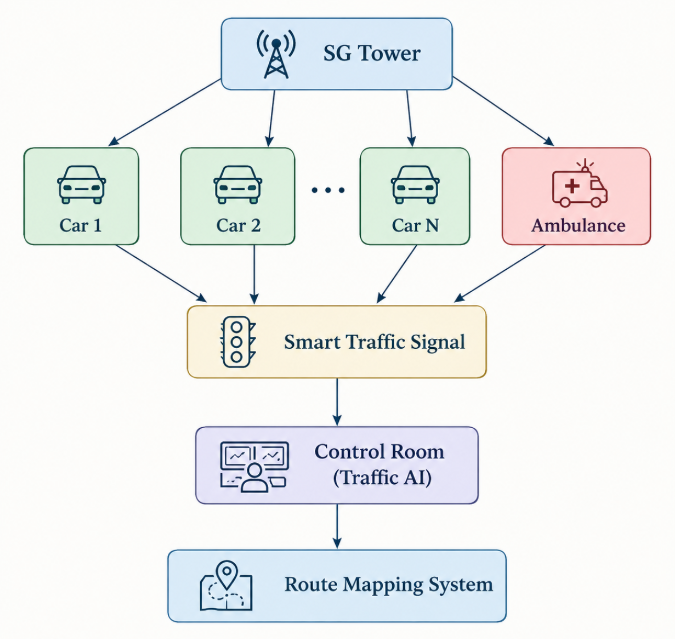
\includegraphics[width=0.72\linewidth,height=0.5\textheight,keepaspectratio]{image-005.png}
\caption{5G-enabled Smart Transportation Systems}
\label{fig:5g-transport}
\end{figure}

\begin{figure}[ht]
\centering
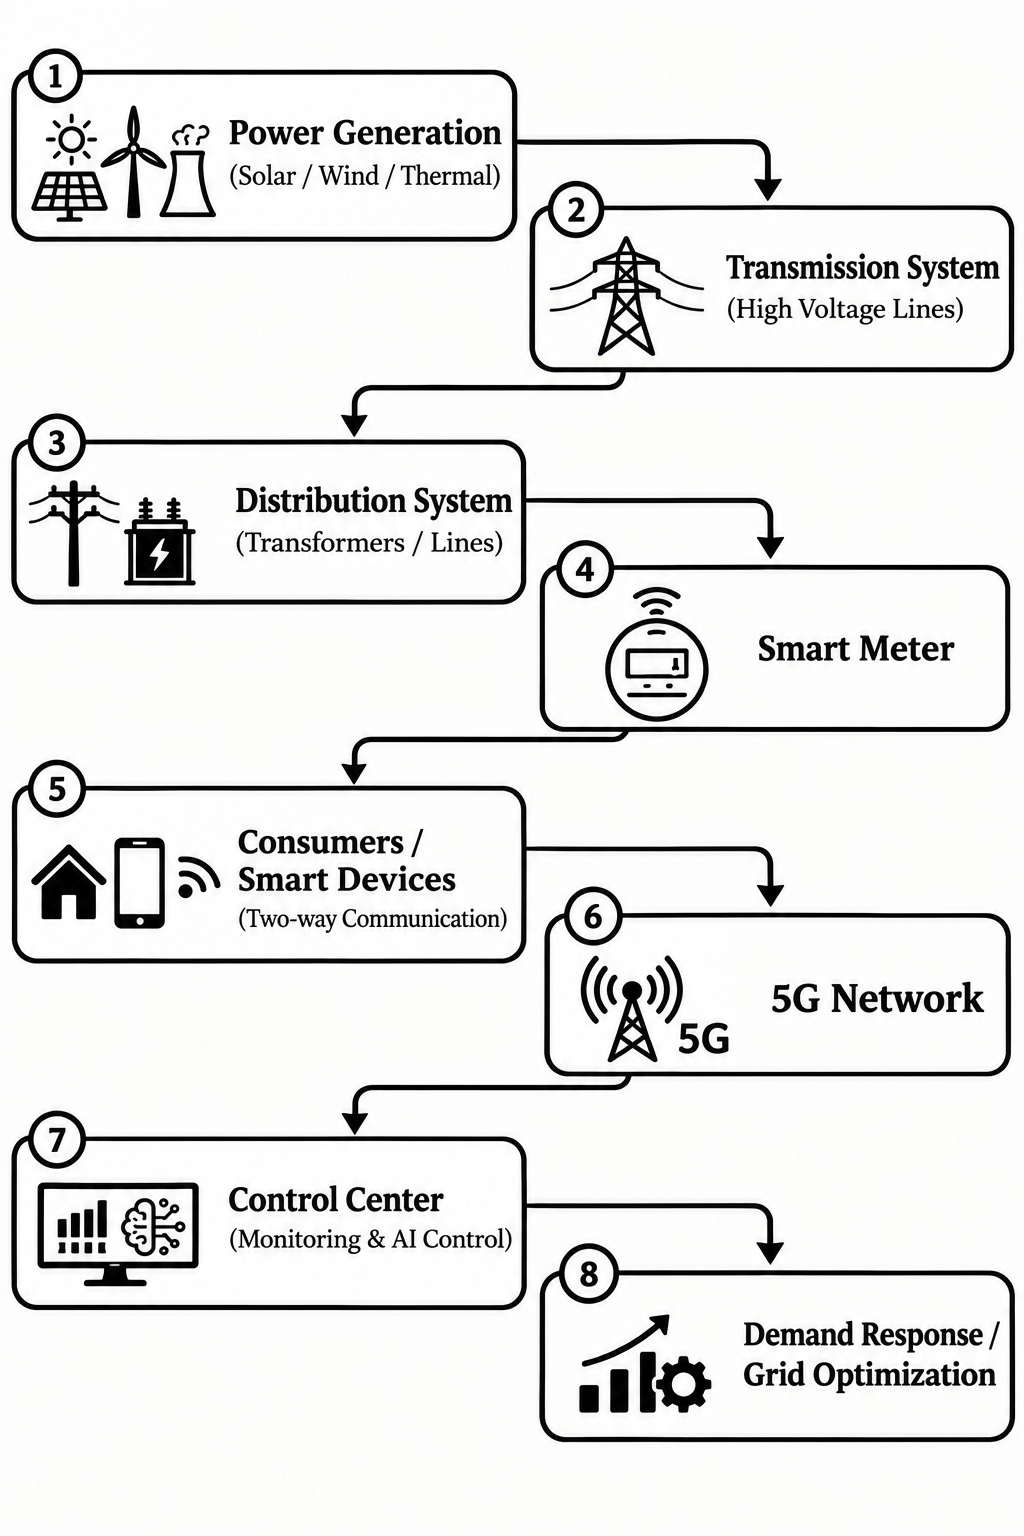
\includegraphics[width=\linewidth,height=0.5\textheight,keepaspectratio]{image-006.png}
\caption{5G Enabled Smart Grid}
\label{fig:5g-connectivity}
\end{figure}

\begin{figure}[ht]
\centering
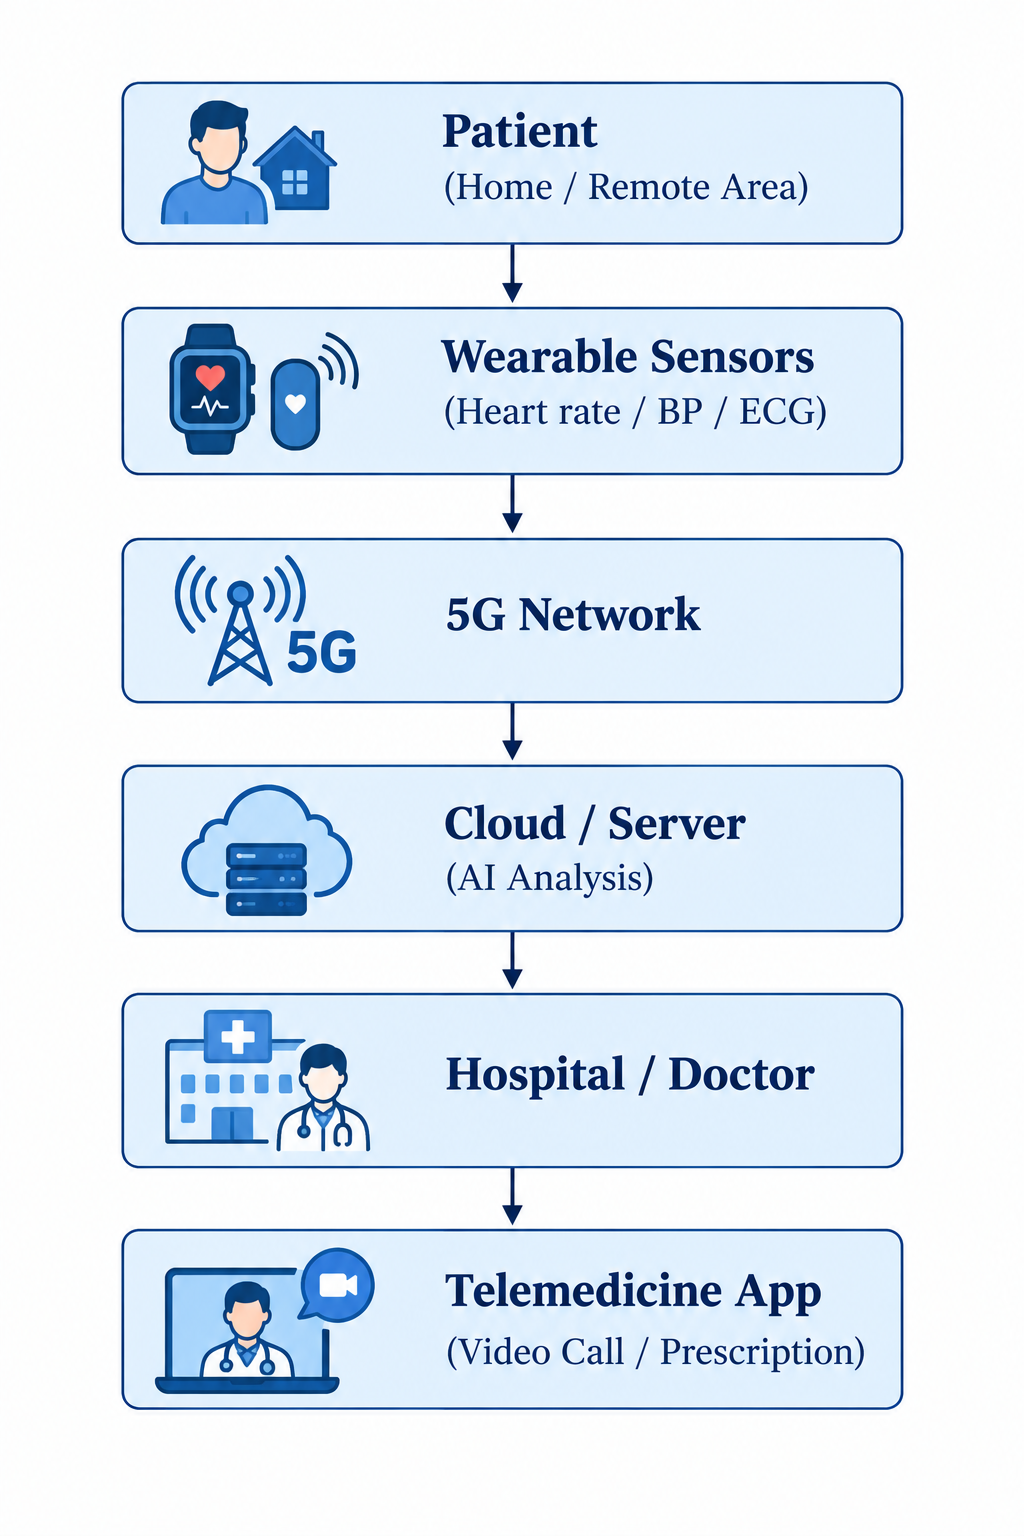
\includegraphics[width=\linewidth,height=0.5\textheight,keepaspectratio]{image-007.png}
\caption{5G-enabled Remote Healthcare}
\label{fig:5g-v2x}
\end{figure}

Vehicle-to-everything (V2X) communication enables connected and automated vehicles to exchange information with other vehicles as well as surrounding road infrastructure. The dependable connectivity and minimal communication delays provided by 5G networks are particularly important for facilitating these exchanges, thereby supporting the safe, coordinated, and efficient operation of autonomous vehicles \cite{r43}.

Pairing smart grids with 5G makes it possible to monitor and control energy systems in real time. Smart grid communication technologies help distribute energy efficiently, bring in renewable power sources, and respond quickly when demand shifts, which makes urban energy systems more sustainable and reliable \cite{r44}. Fig.~\ref{fig:5g-connectivity} shows the architecture of a 5G-enabled smart grid.

5G also strengthens public safety by allowing emergency responders to communicate and coordinate in real time. It supports applications such as remote monitoring, predictive data analysis, and rapid resource mobilization, which help cities respond to emergencies faster and more effectively. Research on public safety communications shows that "5G capabilities can transform emergency response by giving first responders better situational awareness and coordination \cite{r45}, although deployment remains most demanding in densely populated urban centers and areas with limited existing infrastructure. Fig.~\ref{fig:5g-safety} shows a representative 5G-based emergency-response framework.

\begin{figure*}[!t]
\centering
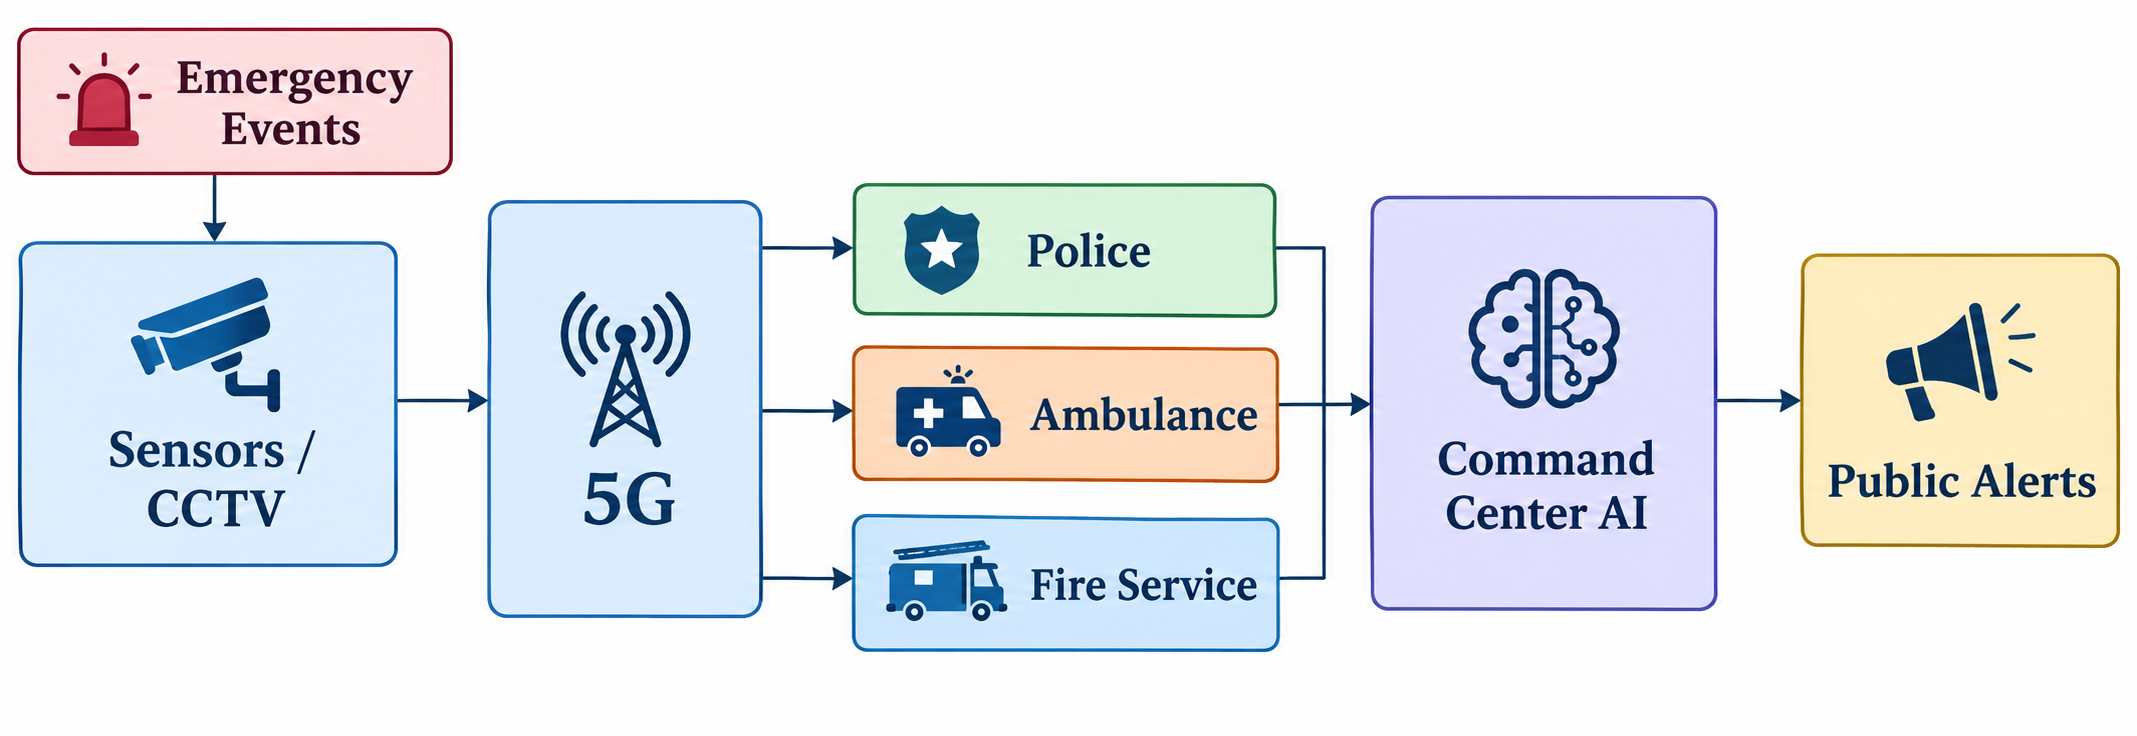
\includegraphics[width=\textwidth]{image-008.png}
\caption{5G for Public Safety and Emergency Response}
\label{fig:5g-safety}
\end{figure*}

5G is also changing healthcare by making telemedicine, remote patient monitoring, and more advanced medical procedures possible. High-definition video consultations, real-time transmission of medical data, and remote-assisted procedures all make healthcare more efficient and easier to reach, which leads to better patient outcomes. Fig.~\ref{fig:5g-v2x} shows a representative 5G-enabled remote healthcare workflow.

5G plays a similar role as an enabler of Industry 4.0 in smart manufacturing. It supports interconnected factories and automated, real-time data analytics that draw on IoT, robotics, and AI to improve production, flexibility, quantity, and quality. By allowing live data exchange and automation across the whole production chain, 5G helps boost productivity in smart manufacturing and industrial automation \cite{r97}. Fig.~\ref{fig:manufacturing} shows the overall data and material flow in a 5G-enabled smart factory.

\begin{figure}[ht]
\centering
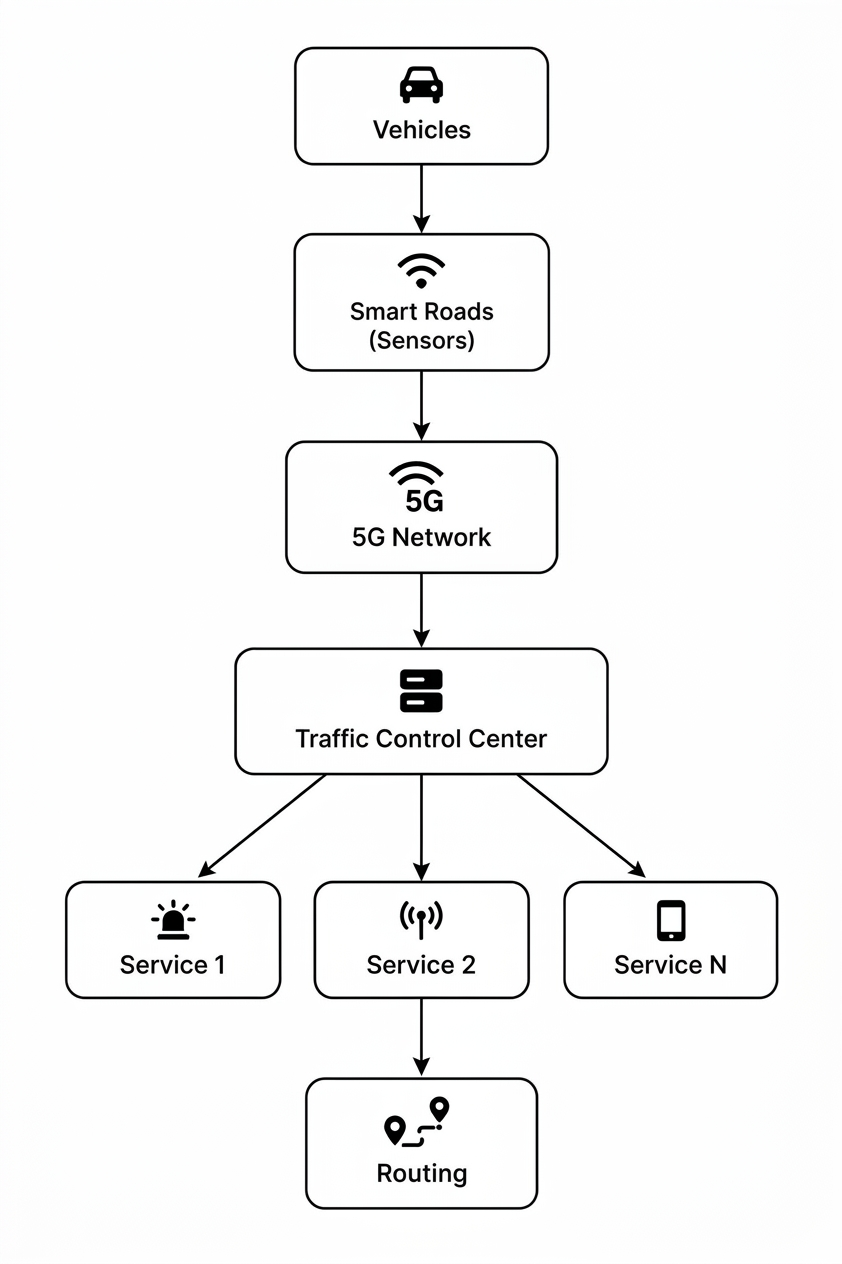
\includegraphics[width=\linewidth,height=0.5\textheight,keepaspectratio]{image-009.png}
\caption{Smart Production and Industry 4.0}
\label{fig:manufacturing}
\end{figure}

Large-scale implementation of 5G networks involves considerable investment in supporting infrastructure, including dense small-cell deployments, fiber-optic backhaul systems, and edge-computing resources, as outlined in Table~\ref{tab:5g}. Effective spectrum planning and allocation are also fundamental to successful 5G implementation, with network deployments utilizing a combination of licensed, shared-access, and unlicensed frequency bands \cite{r37}.

\begin{table}[!t]
\caption{Components of 5G Infrastructure}
\label{tab:5g}
\centering
\scriptsize
\setlength{\tabcolsep}{3pt}
\renewcommand{\arraystretch}{1.15}

\begin{tabularx}{\linewidth}{|
>{\raggedright\arraybackslash}p{0.18\linewidth}|
>{\raggedright\arraybackslash}X|
>{\raggedright\arraybackslash}X|
>{\raggedright\arraybackslash}X|}
\hline

\textbf{Components} &
\textbf{Description} &
\textbf{Role in Smart Applications} &
\textbf{Real-World Examples} \\
\hline

IoT Sensors &
Devices that capture environmental, traffic, and infrastructure data. &
Enable real-time monitoring of traffic, pollution, and public utilities. &
Air quality sensor networks in Barcelona. \\
\hline

Data Centers &
Facilities for processing, storing, and managing large volumes of urban data. &
Support data analytics, decision-making, and service delivery. &
Smart city data hubs in Amsterdam. \\
\hline

Cloud Computing &
Scalable computing resources delivered over the internet. &
Enables large-scale data processing, storage, and smart city applications. &
Cloud-based urban management platforms in Singapore. \\
\hline

Urban Platforms &
Integrated platforms that consolidate data from multiple city departments. &
Facilitate data sharing, visualization, and coordinated decision-making. &
Barcelona Urban Platform; FIWARE-based smart city platforms. \\
\hline

\end{tabularx}
\end{table}

Digital infrastructure is thus anchored by cloud computing, IoT sensors, and data centers, all of which together allow cities to manage themselves efficiently. Sensors monitor continuous traffic and environmental conditions -- air-quality monitoring in Barcelona is a representative example \cite{r39} -- while data centers provide the storage and analysis capacity needed for large-scale urban data, as illustrated by Amsterdam's smart data hubs \cite{r40}. Cloud computing supplies the internet-based, scalable resources that projects such as Singapore's Smart Nation initiative rely on to aggregate data across the city \cite{r41}, and Virtual Singapore's urban data platform offers centralized, real-time visualization that supports inter-departmental coordination for the benefit of residents \cite{r42}. Together, these digital elements are what make contemporary cities smart and sustainable. Fig.~\ref{fig:strategies} presents key strategies for optimizing digital infrastructure.

\begin{figure}[ht]
\centering
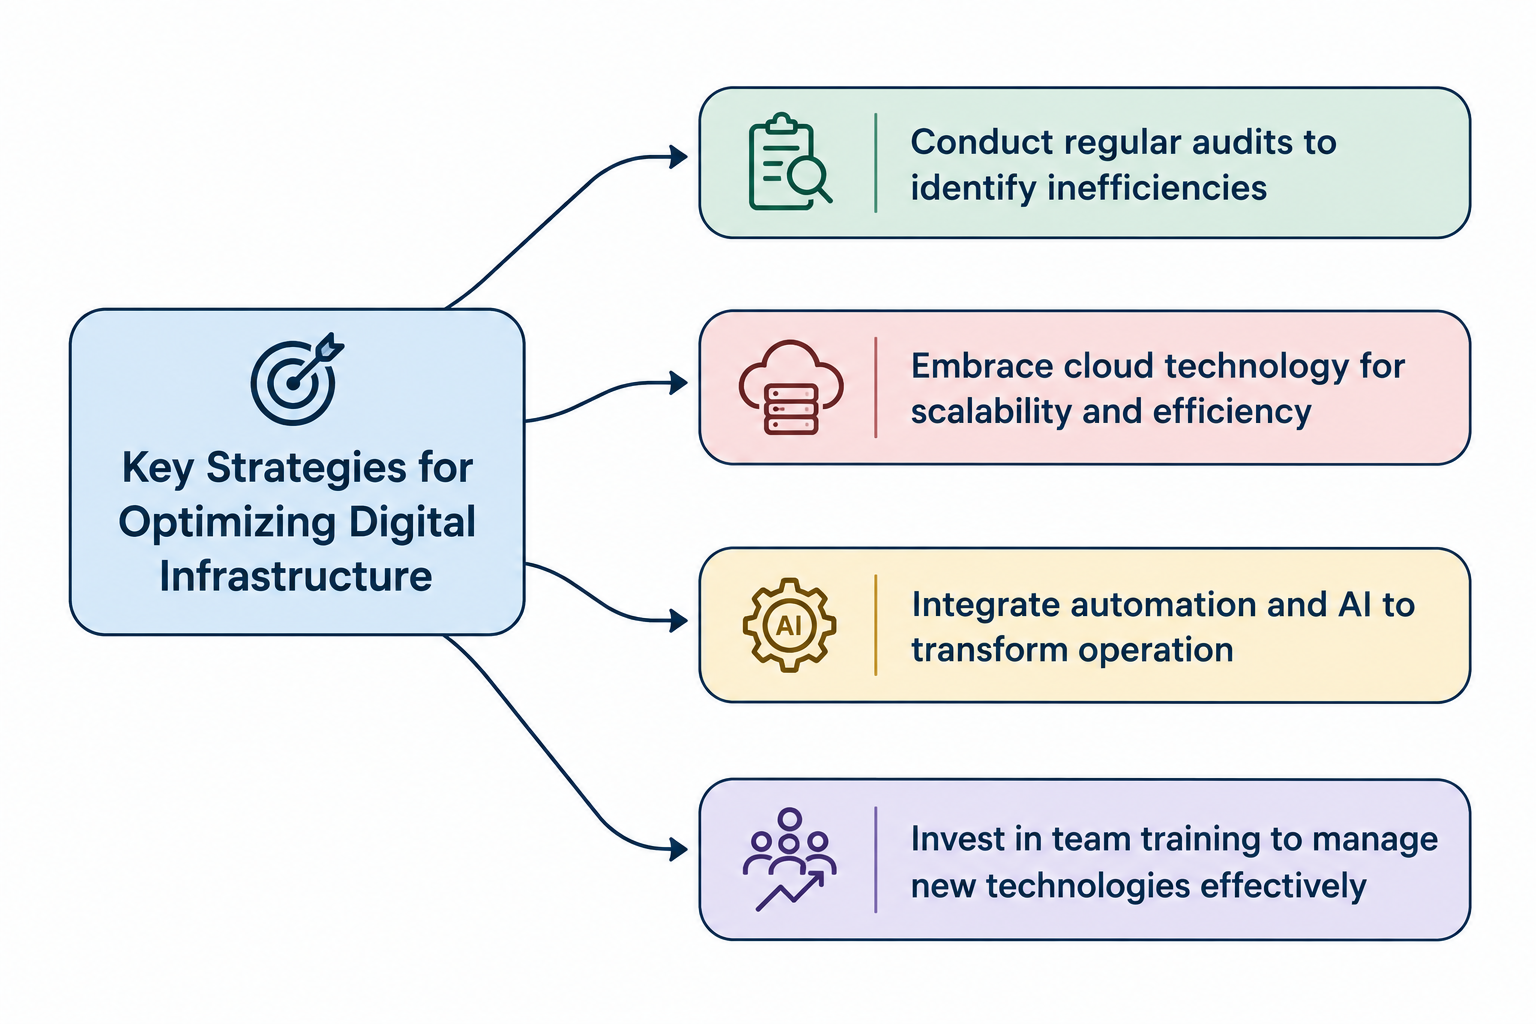
\includegraphics[width=0.8\linewidth]{image-010.png}
\caption{Approaches to Digital Infrastructure Optimization}
\label{fig:strategies}
\end{figure}

\subsection{Physical Infrastructure}
\noindent This part looks at intelligent buildings (HVAC, BMS, EMS), intelligent highways and roads (V2I, adaptive signaling), and smart water and waste management systems as the three dimensions of physical infrastructure modernization.

Updating traditional infrastructure to meet the needs of smart urban environments means bringing in advanced technology that makes operations more efficient, supports environmental sustainability, and improves residents' quality of life. Such modernization is important for responding effectively to the complex challenges associated with urban development while enabling long-term sustainable growth. This subsection focuses on three major dimensions of infrastructure modernization: intelligent buildings, technologically enhanced roads and highways, and upgraded systems for water and waste management.

\subsubsection{Digitally Enabled Buildings}
\noindent This part looks at how HVAC, BMS, and EMS are brought together in intelligent buildings.

Intelligent buildings use advanced digital technologies to control energy use, improve how a building runs, and make indoor spaces more comfortable for the people inside. According to the International Energy Agency (IEA), building operations account for approximately 30\% of global final energy consumption and 27\% to 30\% of total energy-sector $\text{CO}_2$ emissions (rising to nearly 36\% to 40\% when embodied carbon from construction and manufacturing materials is incorporated) \cite{r125}. Consequently, modernizing the built environment is pivotal to urban decarbonization. Intelligent buildings integrate automated solutions to govern illumination, heating, ventilation, air conditioning (\textbf{HVAC}), and security, combining IoT sensor telemetry, edge analytics, and automated control platforms. The primary elements include \textbf{Energy Management Systems (EMS)}, \textbf{Building Management Systems (BMS)}, and environmentally conscious architectural design.

Energy Management Systems track and regulate power distribution and thermal loads in real time, optimizing consumption profiles, minimizing waste, and shaving peak electrical demand. Empirical assessments indicate that deploying smart BEMS, predictive HVAC scheduling, and daylight-responsive lighting controls yields operational energy savings between 10\% and 30\%, with specialized sub-system controls reducing HVAC and lighting loads by up to 30\% to 50\% compared to conventional unautomated baselines \cite{r19,r125}.

Building Management Systems (BMS) bring these varied subsystems, including lighting, \textbf{HVAC}, access control, and fire safety, together under a single control architecture. This centralized setup offers continuous diagnostics, predictive fault detection, and environmental control that responds to the people using the space, which gets the most out of operations while also improving indoor comfort and health.

The Edge in Amsterdam is a good example of this approach. It is one of the most technologically advanced commercial buildings in the world, combining an efficient energy management system, more than 28,000 IoT sensors, automated Power-over-Ethernet lighting, and dynamic climate control, which together deliver net-positive energy performance \cite{r46}. One World Trade Center in New York City follows a similar path, with extensive green technologies, dynamic thermal regulation, and advanced BMS strategies that align with LEED certification principles \cite{r47}.

Intelligent building technologies call for a large upfront investment. Getting different devices and systems to work together takes careful coordination, standardized protocols, and thorough planning. The constant stream of data from building systems also raises privacy and cybersecurity risks, so strong data protection and security measures are needed.

\subsubsection{Intelligent Highways and Roads}
\noindent This part looks at adaptive traffic signaling, V2I communication, and real-time traffic analytics as ways to reduce congestion and improve road safety.

Intelligent road and highway infrastructure brings together sensing technologies, adaptive signaling, and real-time analytics to make traffic run more smoothly, improve safety on the road, and ease congestion. Roadside sensors and surveillance cameras constantly collect information on vehicle flow, travel speeds, and road conditions. This data can then be analyzed to spot traffic patterns, catch congestion as it starts to build, and adjust signal timings automatically to match current conditions, as illustrated in Fig.~\ref{fig:roads}.

\begin{figure}[ht]
\centering
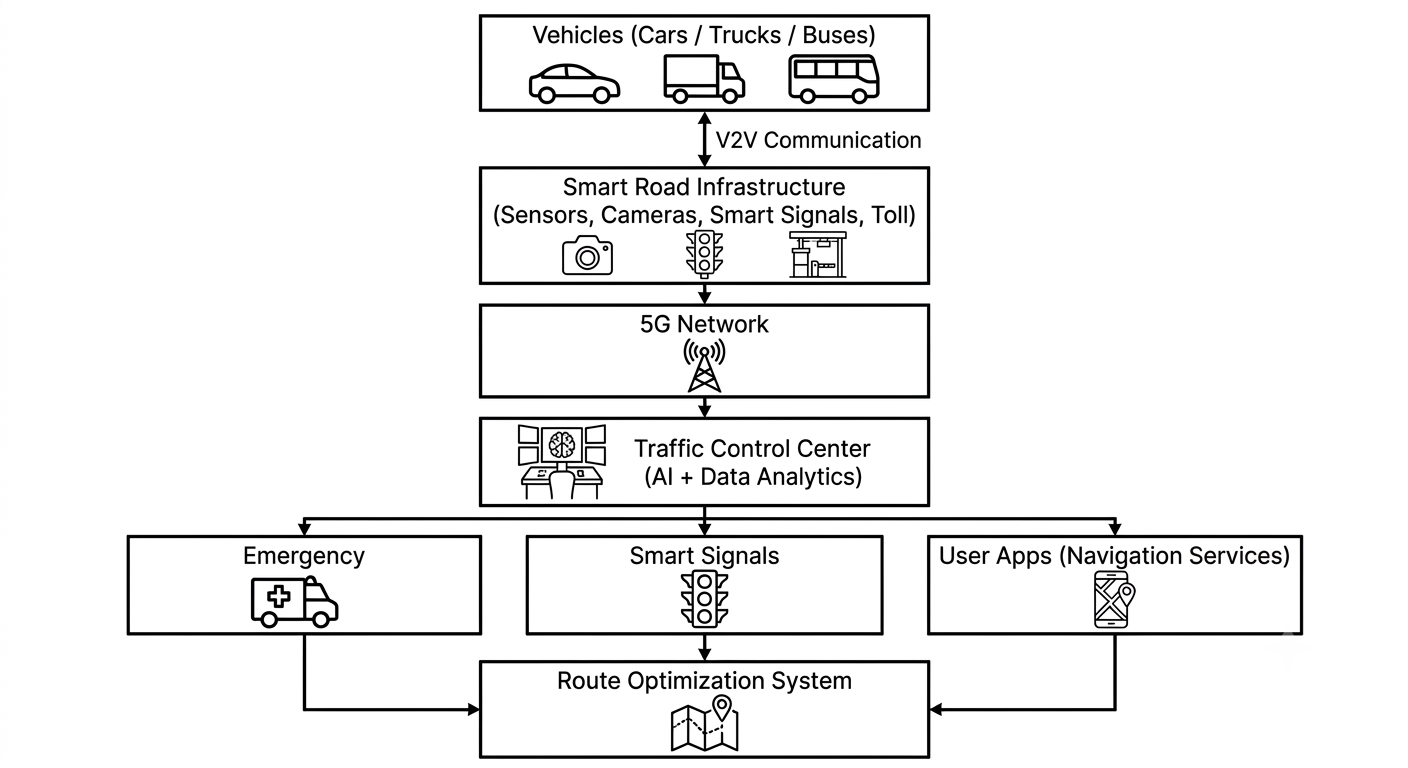
\includegraphics[width=\linewidth,height=0.5\textheight,keepaspectratio]{image-014.png}
\caption{Smart Roads and Highways}
\label{fig:roads}
\end{figure}

Traffic management systems that combine real-time sensing with adaptive control offer decisive advantages in mitigating road network congestion \cite{r48}. Smart traffic signals utilize loop detectors, radar, and video analytics to adjust cycle lengths, phase splits, and green times dynamically in response to prevailing vehicular queues. As synthesized in Table~\ref{tab:asct_performance}, empirical assessments by the U.S. Federal Highway Administration (FHWA) demonstrate that Adaptive Signal Control Technologies (ASCT) cut average commuter travel times and intersection delays by 10\% to 25\%, with improvements exceeding 50\% along severely congested corridors operating on outdated fixed-time schedules \cite{r49,r126}. Furthermore, by smoothing vehicular shockwaves and cutting unnecessary stops by 20\% to 40\%, adaptive control systems reduce idling fuel consumption and tailpipe greenhouse gas emissions ($\text{CO}_2$, $\text{CO}$, and unburned hydrocarbons) by 10\% to 20\% \cite{r126}.

\begin{table}[!t]
\caption{Operational and Environmental Improvements from Adaptive Signal Control Technologies (ASCT) [Source: U.S. Federal Highway Administration (FHWA) \cite{r126}]}
\label{tab:asct_performance}
\centering
\scriptsize
\setlength{\tabcolsep}{3pt}
\renewcommand{\arraystretch}{1.2}
\renewcommand{\tabularxcolumn}[1]{m{#1}}
\begin{tabularx}{\linewidth}{|
>{\raggedright\arraybackslash}m{0.32\linewidth}|
>{\centering\arraybackslash}m{0.22\linewidth}|
>{\raggedright\arraybackslash}X|}
\hline
\textbf{Performance Metric} & \textbf{Observed Gain} & \textbf{Operational Mechanism} \\
\hline
Arterial Travel Time & 10\% to 25\% reduction & Continuous green-band optimization across corridors \\
\hline
Intersection Control Delay & 15\% to 50\% reduction & Eliminates idle wait times along congested arterials \\
\hline
Vehicular Stops & 20\% to 40\% reduction & Dynamic phase extensions accommodate active platoons \\
\hline
Fuel Consumption & 8\% to 15\% reduction & Minimizes stop-and-go cycles and acceleration losses \\
\hline
Tailpipe Emissions & 10\% to 20\% reduction & Lowers idling $\text{CO}_2$, CO, and hydrocarbon exhaust \\
\hline
Corridor Capacity & 5\% to 12\% increase & Dynamic clearance allocates green splits by queue length \\
\hline
Schedule Reliability & 20\% to 35\% gain & Reduces travel time variability for public transit and freight \\
\hline
\end{tabularx}
\end{table}

Vehicle-to-Infrastructure (V2I) communication enables vehicles to exchange information with roadside sensing devices and traffic signal systems, as illustrated in Fig.~\ref{fig:v2i}.

\begin{figure}[ht]
\centering
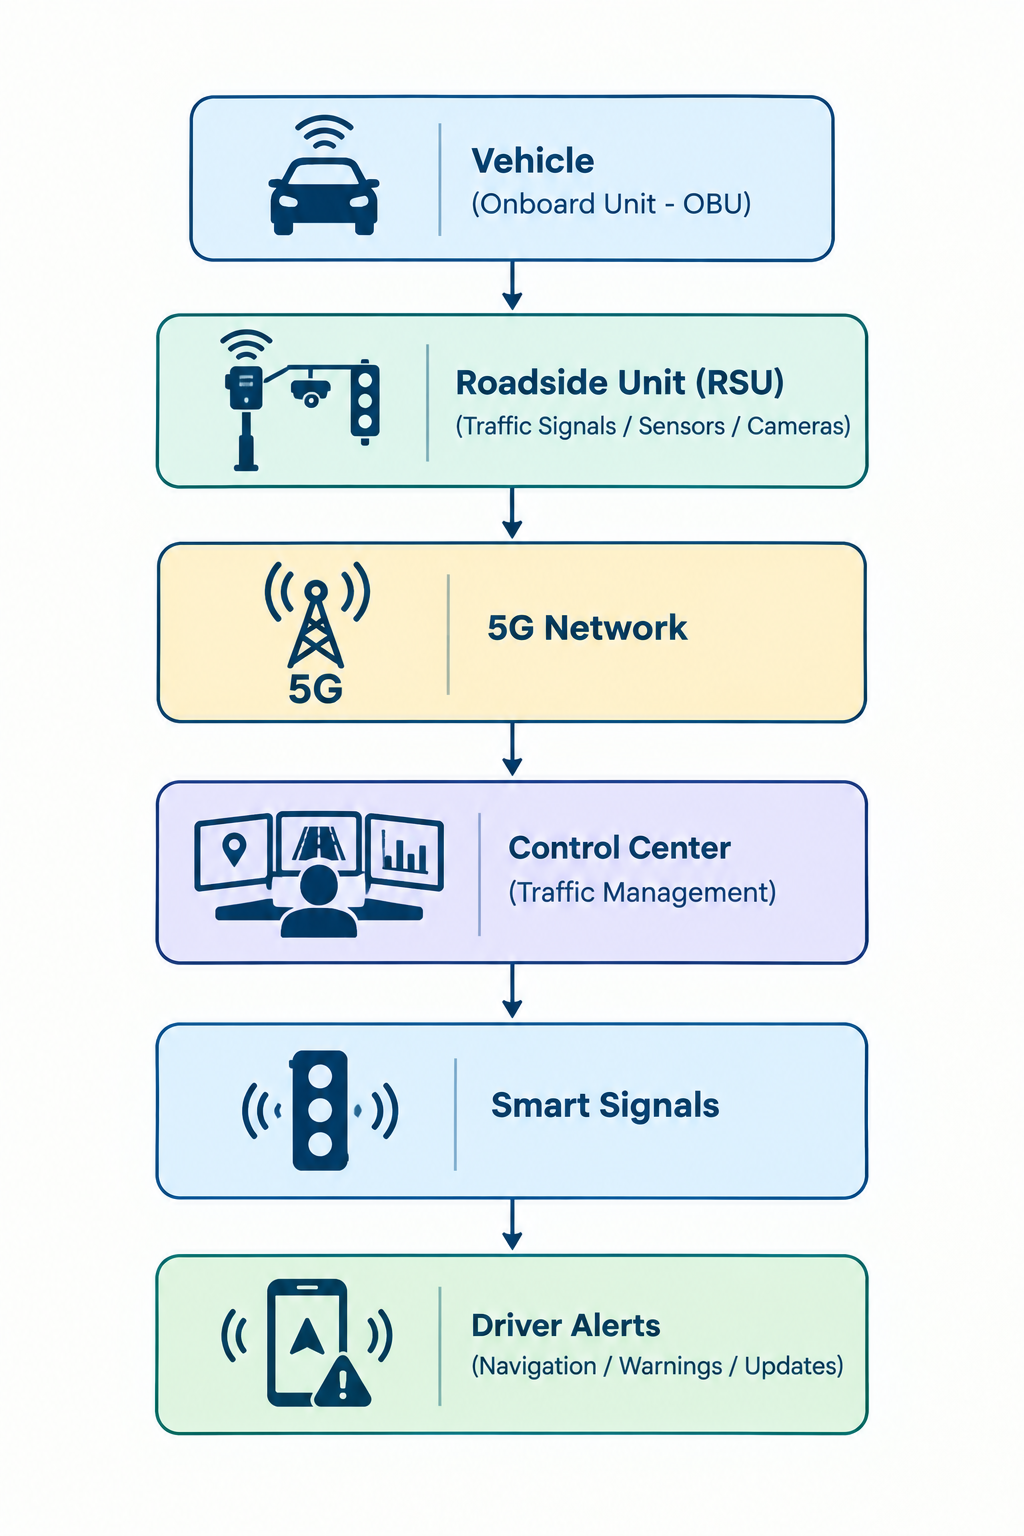
\includegraphics[width=\linewidth,height=0.5\textheight,keepaspectratio]{image-015.png}
\caption{Vehicle-to-Infrastructure (V2I) Communication}
\label{fig:v2i}
\end{figure}

"This technology supports applications such as traffic signal priority, collision avoidance, and real-time route adjustment; V2I communication enhances both safety and efficiency and has the potential to reduce the number of traffic accidents" \cite{r50}. The Los Angeles Smart Corridor exemplifies an integrated traffic management system that combines real-time signal control and dynamic message displays to coordinate freeway and arterial traffic, reducing congestion and travel delays \cite{r51}, while the Barcelona Smart Traffic Management System combines traffic sensors, intelligent signaling, and data analysis to reduce the congestion and improve the flow of traffic in that city \cite{r52}.

Despite their potential benefits, intelligent road and highway systems present several practical challenges. Deployment often requires a large initial investment in technological infrastructure, and collecting and handling so much traffic-related data raises concerns about privacy and data protection. On top of that, making new technologies work with established traffic management infrastructure can be technically complex.

\subsubsection{Waste and Water Management Systems}
\noindent This part looks at smart water metering, leak detection, waste-bin fill-level sensing, route optimization, and advanced treatment (membrane filtration, UV disinfection) as ways to improve water and waste efficiency.

Intelligent water and waste management systems rely on sensors, analytics, and automation to improve how water is distributed and waste is collected, cut pollution, and lessen the impact on the environment, as shown in Fig.~\ref{fig:water}.

\begin{figure}[ht]
\centering
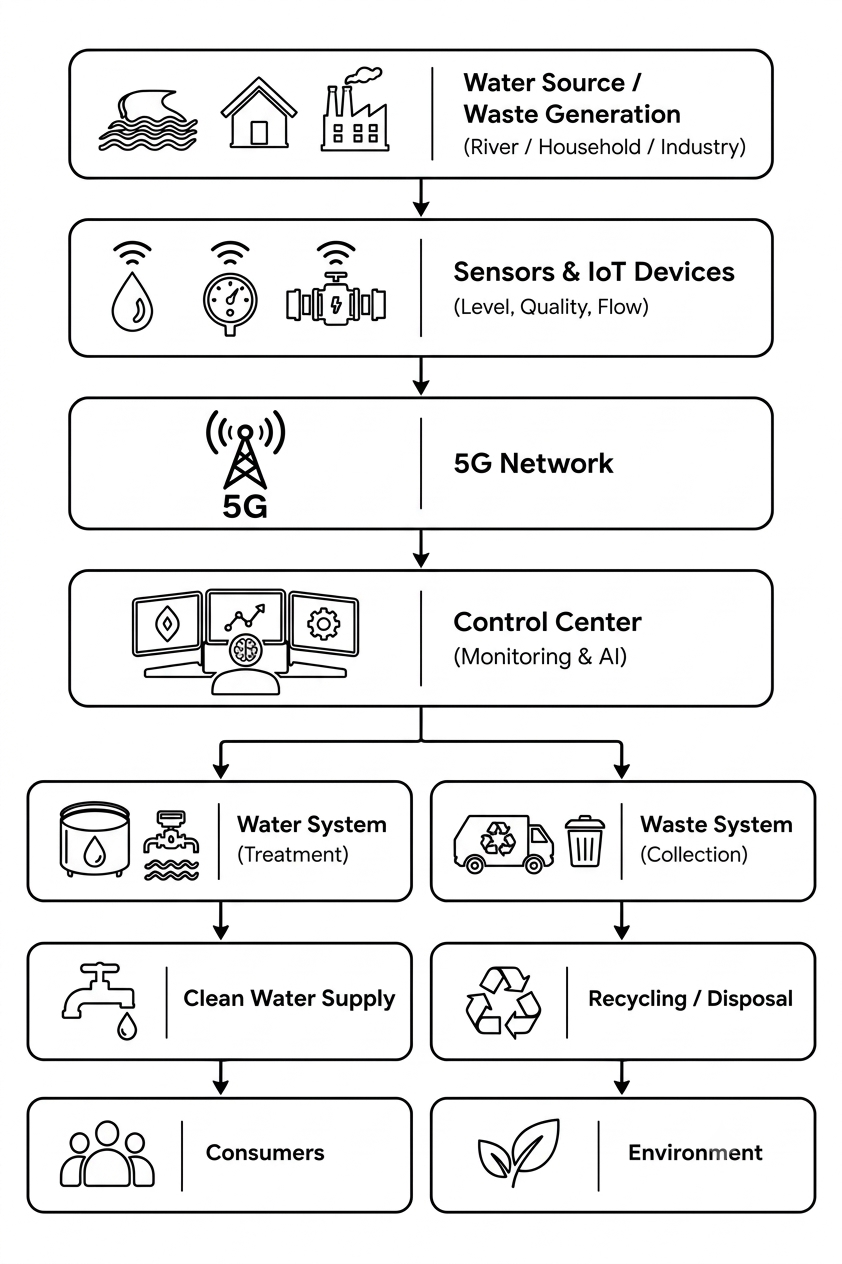
\includegraphics[width=\linewidth,height=0.5\textheight,keepaspectratio]{image-016.png}
\caption{Smart Water and Waste Management Systems}
\label{fig:water}
\end{figure}

Smart water meters provide continuous data on consumption patterns, which supports accurate billing, quick identification of leaks, and better allocation of water resources. As summarized in Table~\ref{tab:nrw_benchmarks}, benchmarks compiled by the World Bank and the International Water Association (IWA) estimate that non-revenue water (NRW) accounts for 32 to 45 billion cubic meters of treated drinking water lost every year around the world, caused by pipe bursts, deteriorating joints, and commercial metering errors. This costs global utilities between \$14 billion and \$40 billion annually \cite{r127}. In developing urban centers, NRW rates often reach 35\% to 50\% (and up to 60\%) of total municipal production. Using Advanced Metering Infrastructure (AMI), permanent acoustic leak detection loggers, and automated District Metered Areas (DMAs) lets utilities cut physical water losses by 20\% to 40\% and bring leak detection down from months to hours \cite{r53,r127}.

\begin{table}[!t]
\caption{Global Non-Revenue Water (NRW) Losses and Smart Network Mitigation Benchmarks [Source: The World Bank and International Water Association (IWA) \cite{r127}]}
\label{tab:nrw_benchmarks}
\centering
\scriptsize
\setlength{\tabcolsep}{3pt}
\renewcommand{\arraystretch}{1.2}
\renewcommand{\tabularxcolumn}[1]{m{#1}}
\begin{tabularx}{\linewidth}{|
>{\raggedright\arraybackslash}m{0.32\linewidth}|
>{\centering\arraybackslash}m{0.24\linewidth}|
>{\raggedright\arraybackslash}X|}
\hline
\textbf{Parameter / Solution} & \textbf{Observed Benchmark} & \textbf{Economic / Environmental Impact} \\
\hline
Global Annual Potable Loss & 32 to 45 Billion $\text{m}^3$ & Equivalent to supplying 90M+ urban households \\
\hline
Global Financial Utility Loss & \$14B to \$40B / year & Drains municipal infrastructure maintenance budgets \\
\hline
NRW in Developing Cities & 35\% to 50\% (peak $>$60\%) & Major impediment to UN SDG 6 clean water targets \\
\hline
NRW in Developed Cities & 15\% to 20\% & Focuses on aging pipe renewal and pressure transients \\
\hline
Acoustic IoT Leak Loggers & 20\% to 40\% loss cut & Pinpoints subsurface ruptures before surface emergence \\
\hline
Leak Detection Cycle & Months $\rightarrow$ 24--48 hours & Automated acoustic telemetry isolates metered sectors \\
\hline
Smart AMI Metering & 15\% to 25\% billing gain & Eliminates under-registration and detects unauthorized use \\
\hline
\end{tabularx}
\end{table}

In the waste-management domain, urban centers face rapidly growing volumes: the World Bank's global waste assessments project that municipal solid waste will rise from 2.01 billion tonnes a year in 2016 to 3.40 billion tonnes by 2050, a 70\% increase driven by fast urbanization and economic expansion. Connected ultrasonic sensors installed in collection bins track fill levels in real time and make it possible to optimize routes for collection fleets. Field deployments show that sensor-guided collection schedules remove redundant trips, cutting municipal collection costs and truck mileage by 20\% to 35\% and reducing diesel emissions along with them \cite{r54,r57}. At water treatment facilities, advanced processes such as membrane filtration, ultraviolet (UV) disinfection, and automated chemical dosing keep drinking water within quality standards while lowering life-cycle treatment costs \cite{r55}.

Singapore has put in place an island-wide smart water grid that uses more than 300 real-time acoustic sensors and analytics platforms across its distribution pipelines. It has reached one of the lowest NRW rates in the world (under 5\%) and allocates resources more effectively as a result \cite{r56}. Rome and Barcelona have likewise set up smart waste systems in which bin fill-level telemetry automates routing, which lowers municipal fuel spending and carbon footprints \cite{r52,r57}.

Rolling out intelligent water and waste management solutions takes substantial investment in supporting infrastructure. Collecting and processing the data these systems generate also raises important privacy and cybersecurity questions, and these need to be built into the modernization of existing infrastructure and services.

\subsection{Urban Design and Planning}
\noindent This part looks at mixed-use developments (energy, transport, waste), green infrastructure (parks, corridors, urban forests), and sustainable urban development (renewables, rainwater, passive solar) as planning dimensions for livable cities.

Bringing intelligent technologies into urban planning helps shape cities that are efficient, sustainable, and pleasant to live in. Modern digital solutions let municipalities make better use of the built environment, improve residents' well-being, and deal with new urban challenges. In practice, this means building smart technologies into mixed-use developments, green-space planning, and sustainable approaches to urban development.

\subsubsection{Mixed-Use Developments}
\noindent This part looks at how residential, commercial, and recreational functions are combined with smart energy, transport, and waste systems, using Hudson Yards (NYC) and Marina Bay Sands (Singapore) as case studies.

Smart-enabled mixed-use developments put residential, professional, commercial, and recreational functions together in one shared urban setting. This arrangement makes essential facilities easier to reach, reduces the need to travel, and supports more sustainable ways of living in the city. By mixing different activities with intelligent technologies, these developments add to the convenience, efficiency, and quality of life that smart urban environments aim for.

These developments include integrated infrastructure, such as intelligent energy networks, advanced transportation systems, and coordinated waste-management facilities, to make cities run more efficiently while limiting environmental harm. Studies of land-use and transportation patterns suggest that mixed-use planning can shorten commuting distances, which helps ease traffic congestion and cut greenhouse gas emissions \cite{r58}. Inside these developments, smart buildings use automated controls to manage energy consumption, lighting, and \textbf{HVAC} systems, which makes occupants more comfortable while lowering operating costs and supporting sustainability goals. Research on building energy consumption has shown that such intelligent systems can raise energy efficiency considerably while reducing operating expenses \cite{r59}. Mixed-use environments can also include sustainable mobility options, such as electric vehicle charging infrastructure, bicycle-sharing services, and integrated public transit, which give people alternatives to driving. Studies of mixed-use development suggest that offering these options, especially public transportation and bicycle-sharing, can reduce reliance on personal vehicles \cite{r60}.

Hudson Yards in New York combines modern building management, energy-saving infrastructure, and smart mobility, turning the neighborhood into a modern district with shorter commutes \cite{r61}. Marina Bay Sands in Singapore brings together residential, commercial, and entertainment functions with energy-efficient infrastructure, intelligent transport, and integrated systems that improve urban life and sustainability \cite{r62}. Table~\ref{tab:mixed} summarizes key findings on mixed-use development across countries.

\begin{table*}[!t]
\caption{Key Findings of Mixed-Use Developments in Various Countries}
\label{tab:mixed}
\centering
\scriptsize
\setlength{\tabcolsep}{3pt}
\renewcommand{\arraystretch}{1.15}

\begin{adjustbox}{width=\textwidth}
\begin{tabularx}{\textwidth}{|
>{\centering\arraybackslash}p{0.05\textwidth}|
>{\raggedright\arraybackslash}X|
>{\raggedright\arraybackslash}X|
>{\raggedright\arraybackslash}X|
>{\raggedright\arraybackslash}X|
>{\raggedright\arraybackslash}X|
>{\raggedright\arraybackslash}X|}
\hline

\textbf{Ref} &
\textbf{Study Area / Country} &
\textbf{Type of Development} &
\textbf{Key Components} &
\textbf{Smart Technologies Used} &
\textbf{Key Findings} &
\textbf{Limitations} \\
\hline

{[73]} &
Global &
Mixed-use urban developments &
Residential, commercial, public spaces &
Smart infrastructure, energy systems &
Improves sustainability, economic activity &
Lacks real-time implementation data \\
\hline

{[74]} &
Europe &
Mixed-use projects &
Housing, offices, retail &
Urban planning tools &
Enhances social interaction, land efficiency &
Policy complexity \\
\hline

{[75]} &
Asia / Global &
Urban megaprojects &
Multi-functional urban zones &
Smart planning frameworks &
Large-scale mixed-use improves urban efficiency &
High cost, long timelines \\
\hline

{[76]} &
Global &
Smart city development &
Integrated urban systems &
IoT, data analytics, cloud &
Sustainability + smart governance &
Data privacy concerns \\
\hline

{[77]} &
Global &
Smart sustainable cities &
Infrastructure + services &
IoT, AI, big data &
Improves resource optimization &
Implementation complexity \\
\hline

{[78]} &
Global &
Research trends &
Urban systems &
Digital technologies &
Growing focus on sustainability \& mixed-use &
Limited empirical validation \\
\hline

{[79]} &
Europe &
Smart construction &
Real estate + infrastructure &
Industry 4.0, IoT &
Smart construction supports mixed-use growth &
Technology adoption barriers \\
\hline

{[80]} &
Middle East &
Smart housing &
Residential + community services &
Smart home tech, energy systems &
Enhances quality of life &
Cost constraints \\
\hline

{[81]} &
Global &
Smart city frameworks &
Urban planning systems &
ICT, governance platforms &
Mixed-use is core to smart urbanism &
Conceptual focus \\
\hline

{[82]} &
Global &
Compact urbanism &
Dense mixed land use &
Data-driven planning &
Supports sustainability \& mobility &
Limited case-specific analysis \\
\hline

\end{tabularx}
\end{adjustbox}
\end{table*}

Mixed-use development has its limits, including land-use conflicts, economic uncertainty, and the difficulty of managing several functions within one project. The up-front cost of smart technologies and mixed-use planning is high, and developers and municipalities also have to work through complex zoning rules and approval processes that can hold projects up.

\subsubsection{Green Infrastructure and Sustainable Urban Development}
\noindent This part looks at green corridors, parks, and urban forests for temperature regulation and stormwater management, along with renewable resources, rainwater collection, passive solar design, and green construction principles.

Green spaces are a core part of sustainable urban design. They make cities more livable and improve environmental quality by cutting pollution, regulating temperature, and supporting biodiversity in fast-growing urban areas. Adding green corridors, parks, and urban forests benefits both human well-being and ecological balance, and it helps build healthier, smarter, and more resilient cities that use resources efficiently while protecting natural systems, improving air quality, easing urban heat islands, and giving residents places to relax. Research confirms that urban greening helps regulate urban temperatures and reduce stormwater runoff \cite{r63}. This design approach also puts weight on renewable resources, waste reduction, and green construction, and it draws on principles such as rainwater collection, passive solar design, and the use of renewable energy.

% Plot
\begin{figure*}[!t]
\centering
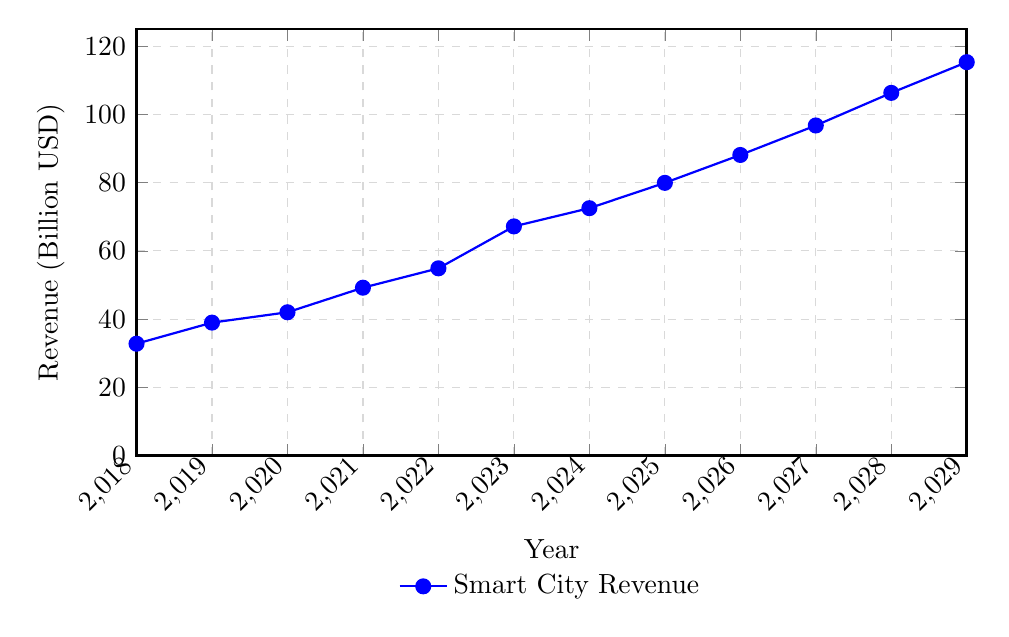
\begin{tikzpicture}
\begin{axis}[
    width=\textwidth,
    height=7cm,
    xlabel={Year},
    ylabel={Revenue (Billion USD)},
    xmin=2018,
    xmax=2029,
    ymin=0,
    ymax=125,
    xtick={2018,2019,2020,2021,2022,2023,2024,2025,2026,2027,2028,2029},
    xticklabel style={rotate=45, anchor=east},
    ytick={0,20,40,60,80,100,120},
    grid=major,
    grid style={dashed,gray!30},
    line width=1pt,
    mark size=2.5pt,
    enlargelimits=false,
    legend style={
        at={(0.5,-0.25)},
        anchor=north,
        draw=none
    }
]

\addplot[
    blue,
    thick,
    mark=*,
    mark options={fill=blue}
] coordinates {
    (2018,32.81)
    (2019,38.99)
    (2020,42.02)
    (2021,49.22)
    (2022,54.9)
    (2023,67.18)
    (2024,72.52)
    (2025,79.94)
    (2026,88.11)
    (2027,96.75)
    (2028,106.3)
    (2029,115.3)
};

\addlegendentry{Smart City Revenue}

\end{axis}
\end{tikzpicture}

\caption{Revenue for Smart Cities from 2018 to 2029 [Source: Statista Market Insights \cite{r130}].}
\label{fig:smartcityrevenue}

\end{figure*}

Buildings and the wider built environment account for roughly 30\% of global final energy consumption and over a quarter of global energy-sector $\text{CO}_2$ emissions. This makes passive solar architecture, biophilic urban design, and energy-efficient retrofitting critical tools for reducing a city's climate impact \cite{r64,r125}. Green spaces also bring significant health benefits, since they support psychological well-being, ease stress, and encourage regular physical activity. Research has also linked access to such environments with fewer symptoms of anxiety and depression \cite{r65}.

The High Line, an elevated linear park built along a former industrial corridor in New York City, shows how green infrastructure can improve a city's appearance, provide space for recreation, and boost local economic growth \cite{r66}. The Vauban district in Freiburg, Germany, brings car-free transit, green space, and low-energy buildings together into a single, coherent sustainable district \cite{r67}. The long-term success of such projects depends on developing green spaces and environmentally friendly buildings capable of withstanding both regional climate conditions and the broader pressures of global warming. Table~\ref{tab:mixed} and Figure~\ref{fig:smartcityrevenue} together illustrate the economic and environmental influence of these policies.

\section{Technological Innovation in Smart Urban Environments}
\noindent This part looks at IoT, Big Data Analytics, AI, blockchain, smart governance, smart mobility, and smart energy systems as the core technological innovations reshaping urban life.

Rapid population growth continues to drive demand for better infrastructure, resource management, and sustainability, and latest technology -- artificial intelligence, the IoT, big data , and cloud processing -- are central to making cities more efficient, responsive, and sustainable in response. These technologies support the collection and interpretation of continuous information and the decision-making that follows, improving sectors as varied as healthcare, transportation, energy, and public safety. This section examines how innovation and technology are set to reshape the future of urban life.

The scale at which these technologies can gather, analyze, and act on data improves decision-making, trend forecasting, and overall urban functionality across public safety, transportation, and city management. Innovation in smart cities goes beyond simply deploying new technologies. It also means rethinking traditional infrastructure and public services in smarter ways. Examples include smart grids that optimize energy distribution, waste-management solutions built to increase recycling, and intelligent transportation systems that help manage and reduce urban congestion. Digital platforms for citizen engagement also let residents talk to municipal authorities in real time, give feedback, and take part in public decision-making. These participatory tools can strengthen community involvement and help make sure smart city initiatives reflect the needs and preferences of the people they serve. Technological innovation also drives economic development in smart cities by attracting capital, creating jobs, and opening the door to new industries, even as the broader push for efficiency, sustainability, and resilience has to deal with global challenges such as social inequality, climate change, and resource depletion.

\subsection{Information and Communication Technology}

ICT lies an important part of smart city operations, allowing data to be collected, processed, and delivered efficiently to improve city management and decision-making. Barcelona has been a leader in integrating ICT into its smart urban programs, deploying a comprehensive urban platform that combines data sources ranging from social media to sensor networks to track and provide urban services such as collection of waste, traffic management, and energy consumption tracking. This integration has produced significant reductions in energy and water use and helped position Barcelona at the prominent of smart city innovation internationally \cite{r68}.

\subsection{Smart City Systems}
\noindent This part looks at IoT sensor networks, big data analytics (NYC Domain Awareness, waste management), AI (City Brain, machine learning), and blockchain (Dubai governance, smart contracts) as the core system technologies behind smart cities.

The Internet of Things (IoT) is a network of connected sensors and devices that collect and share data on urban conditions such as traffic, air quality, and energy use. Because it allows continuous monitoring and management of infrastructure, IoT helps municipal authorities catch problems early, react to changing conditions, and use resources more effectively.

IoT-based dimming systems show what this can look like in practice, turning ordinary lighting into a smart, adaptive, and energy-efficient system. By combining sensors, controllers, and cloud intelligence, this kind of lighting adjusts to real-world conditions, which greatly reduces energy use while making things more comfortable for users. Fig.~\ref{fig:iot-dimming} shows a representative IoT-based smart lighting architecture.

\begin{figure}[ht]
\centering
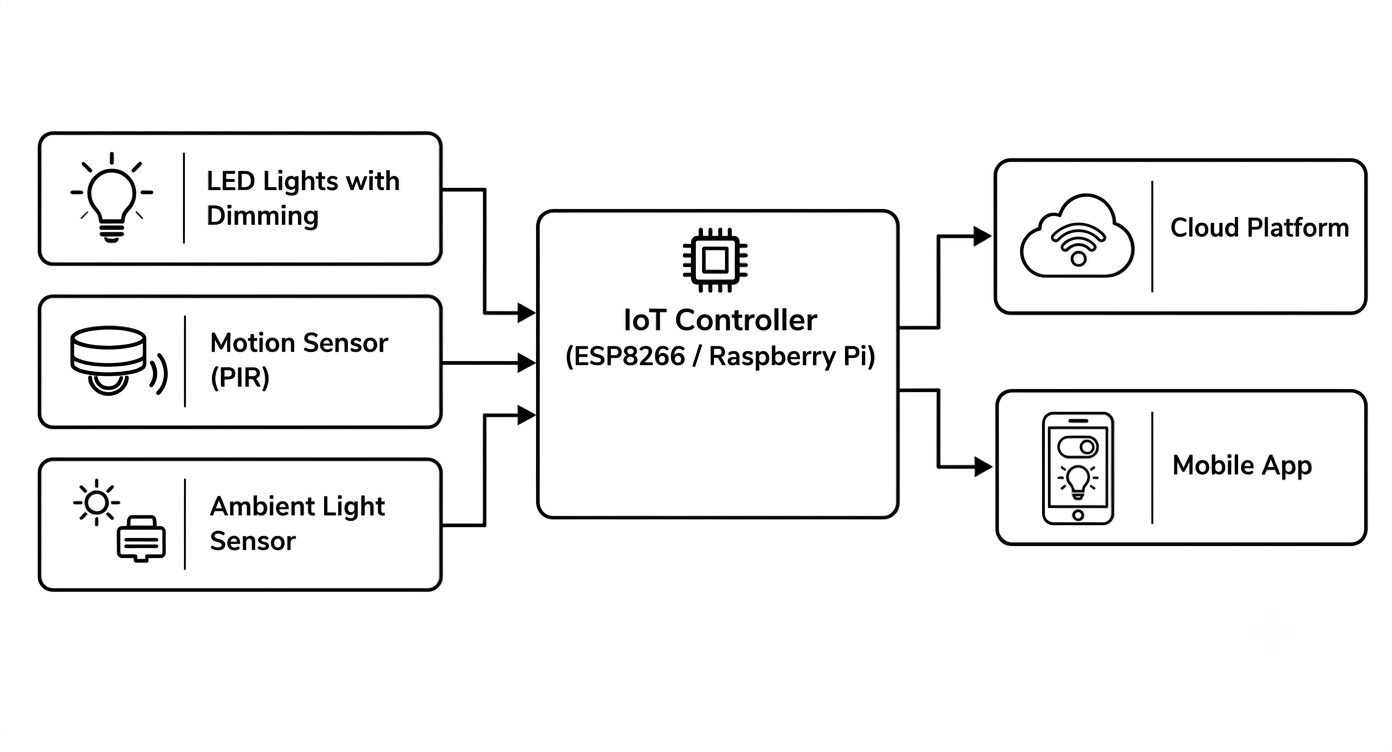
\includegraphics[width=\linewidth]{image-011.png}
\caption{IoT-based Smart Lighting (Dimming) System}
\label{fig:iot-dimming}
\end{figure}

Singapore's Smart Nation initiative is a practical example of smart city implementation, with IoT technologies used to monitor and manage urban infrastructure more effectively. One key application is a nationwide sensor network that tracks traffic conditions and waste-bin fill levels across the city, producing information that can support urban planning and municipal services. Alongside this, AI-driven traffic management approaches have been proposed and tested as a way to tackle congestion on Singapore's road network \cite{r69}.

Big Data Analytics lets cities pull useful insights out of the huge volumes of data generated across sectors, spotting trends and patterns that improve urban services and inform decisions. Applications range from emergency response and energy distribution to traffic forecasting, and officials increasingly rely on data from social media, sensors, and municipal databases.

Municipalities around the world are adopting Big Data Analytics to improve infrastructure management, healthcare, and urban planning. New York City uses analytics to improve the performance of its municipal agencies and support public safety. Its Domain Awareness System combines social media, law-enforcement databases, and CCTV networks for real-time monitoring and incident response \cite{r18}. Big data techniques have also made waste collection more efficient and improved recycling \cite{r70}.

AI builds on IoT and Big Data Analytics by turning the large amounts of data from connected urban systems into insights that can be acted on. AI-enabled solutions support continuous observation, forecasting, and automated operations, which improves the efficiency and sustainability of smart governance, mobility, environmental management, healthcare, and economic activity. Case studies from around the world show AI being used through machine learning, deep learning, and computer vision, and it is increasingly built into many smart city applications. AI therefore acts as an overarching technology that links multiple parts of smart urban ecosystems, although putting it into practice raises challenges around data privacy, infrastructure cost, and common standards \cite{r6}.

Hangzhou, China, home to Alibaba's headquarters, has deployed an AI-enabled "City Brain" system to manage urban infrastructure. The platform processes information collected from more than 1,000 cameras and sensors spread across the city. The results include smoother traffic flow, less congestion, faster emergency response, and better public safety \cite{r71}.

Blockchain technology offers a secure, decentralized platform for managing data transparently without intermediaries. It has become an important part of smart city infrastructure by strengthening data security, trust, and coordination among stakeholders, including governments, developers, and citizens \cite{r92,r93}. Blockchain also works well with the Internet of Things, supporting secure communication and fast data exchange across city-level infrastructure \cite{r94}. In mixed-use developments, blockchain can make operations more efficient through smart contracts, secure property transactions, and energy management systems \cite{r95,r97}. Even so, high implementation costs, scaling challenges, and regulatory uncertainty still hold back its adoption in large-scale smart city projects \cite{r97,r96}.

Dubai has announced a strategy to become a fully blockchain-based government and has already deployed the technology in sectors including healthcare, transportation, and real estate. The Dubai Land Department, for instance, uses blockchain to speed up real estate transactions, cutting the time needed to close a deal from weeks to a few hours, while blockchain has also improved "the transparency and security of the city's digital identity management system" \cite{r72}. This gradual rollout is reflected in how capital is allocated across sectors and how fast markets are growing. As shown in Fig.~\ref{fig:investments} and Fig.~\ref{fig:growth}, foundational domains such as AI, IoT, and big data take the largest share of municipal technology investment and are projected to grow fastest.

\begin{figure*}[!t]
\centering
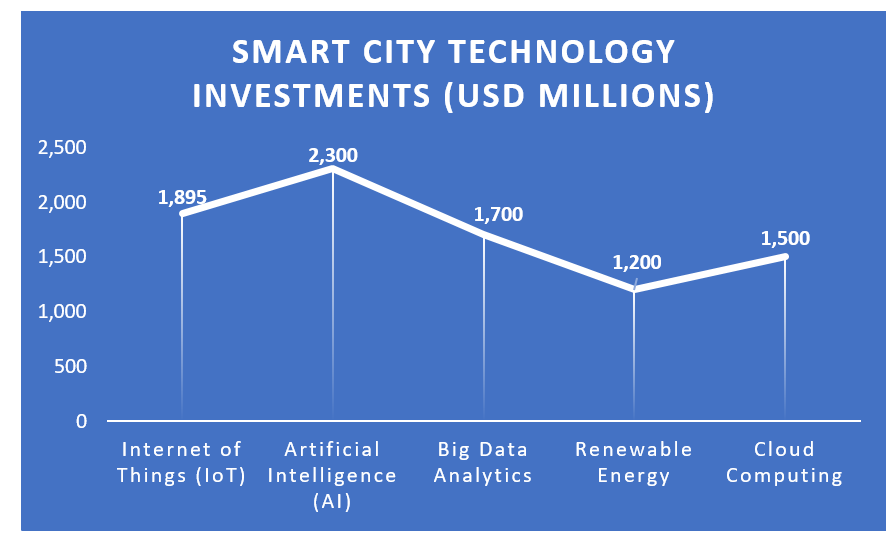
\includegraphics[width=0.8\textwidth]{image-012.png}
\caption{Investments in Smart City Technologies by Sector [Source: IDC Worldwide Smart Cities Spending Guide \cite{r131}].}
\label{fig:investments}
\end{figure*}

\begin{figure*}[!t]
\centering
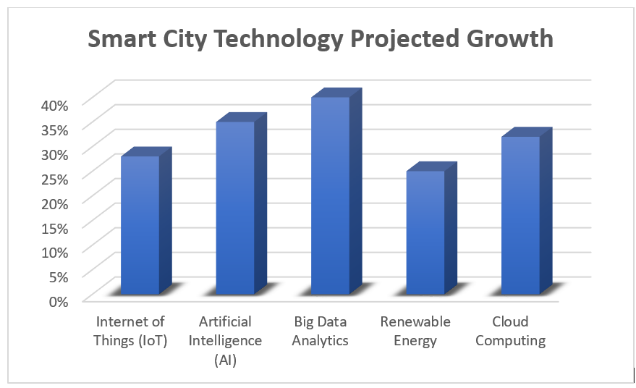
\includegraphics[width=0.8\textwidth]{image-013.png}
\caption{Projected Growth Rate of Smart City Technologies by Sector [Source: Grand View Research and Statista Market Forecast \cite{r132}].}
\label{fig:growth}
\end{figure*}

Smart governance uses technology to improve government operations, reflecting how inclusive, effective, transparent, and participatory a city's decision-making is. Digital platforms let governments broaden citizen participation, streamline administration, and deliver services more effectively. This includes digitizing public services, using data analytics for policy, and integrating citizen feedback into governance.

Authorities routinely draw on live data from multiple sources to handle resources, evaluate municipal infrastructure, and tackle emerging problems, while smart governance further promotes transparency by making government data publicly available and allowing citizens to track program progress -- an openness that builds trust between citizens and government by creating a genuinely participatory governance process.

Seoul, South Korea, has integrated technology across every facet of its city management through a smart governance system that offers more than 1,000 datasets on its Open Data Plaza, allowing citizens to track government activity and engage in policy discussion. Seoul residents can also vote directly on municipal issues through the mVoting smartphone application; together, these initiatives have driven public participation in governance activities above 50 percent \cite{r99,r34}.

E-government services use digital platforms to provide residents with access to public services, while reducing administrative complexity, expanding accessibility, and enabling faster service delivery. By digitizing government functions, smart cities give citizens an easier, more efficient way to engage with government entities, whether through online tax filing, permit applications, or requests for social services. This transition saves time for both citizens and government workers by eliminating the need for in-person office visits, while also ensuring that residents in rural or underserved areas -- and citizens generally, given round-the-clock access -- can obtain the services they need with greater freedom and convenience \cite{r73,r100}.

Estonia, widely regarded as the most technologically advanced e-government in the world, exemplifies this model. Through the e-Estonia project, residents can use multiple services such as voting and tax forms entirely online, and nearly all public services can be completed digitally, saving the government money while giving residents faster, more effective access to public services \cite{r74,r101}.

Citizen participation platforms represent another category of digital technology that enables residents to collaborate with local governments, raise concerns, and take part in decision-making. Digital participation platforms, including social media channels, mobile applications, and web-based discussion forums, let residents contribute to urban governance and can help bring planning decisions in line with community priorities and expectations. These tools set up direct, two-way interaction between citizens and government authorities, so public concerns can be raised, acknowledged, and taken into account in municipal decision-making.

Better Reykjavik is a prominent example of digital citizen engagement in urban governance. Launched in 2010, the platform lets residents submit proposals, discuss possible improvements, and vote on ideas about the city. Proposals that win strong public support are then reviewed by the municipal council and put into practice when they are judged feasible. By 2023, more than 75\% of Reykjavik's population had registered on the platform, and over 800 citizen-originated initiatives had been implemented. This participatory model has added to transparency and raised public trust in municipal administration \cite{r75,r102}.

Smart mobility brings together digital technologies and innovative transport solutions to build urban mobility systems that are efficient, seamless, and environmentally sustainable. Applications include autonomous vehicles, intelligent public transit, and shared mobility services, which ease congestion, limit environmental impact, and improve the travel experience. As a core part of smart urban development, smart mobility also drives economic activity, cuts pollution, and improves quality of life.

Autonomous vehicles (AVs) are self-operating transportation systems that combine advanced sensors, artificial intelligence, and communication technologies to navigate urban roads with limited or no direct human control. In smart cities, they are meant to relieve traffic congestion, reduce road accidents, and make better use of existing road infrastructure. AVs communicate with nearby vehicles, adaptive traffic signals, and centralized urban systems, which lets them process real-time information, find suitable routes, coordinate vehicle movement, and respond to changing traffic conditions as they happen. By reducing dependence on human driving decisions, these systems can tackle a major cause of road accidents while keeping appropriate spacing between vehicles and reacting quickly to unexpected obstacles. Autonomous vehicles can also be built into public transportation networks and shared mobility services, giving further chances to improve the efficiency and coordination of urban transport.

Phoenix, Arizona, has become a major location for autonomous vehicle trials in the United States. Waymo, a subsidiary of Alphabet Inc., has run self-driving vehicles in the city since 2017, using lidar, radar, and camera-based sensing to navigate on their own. The deployment has produced encouraging results for traffic safety and mobility. Analyses of Waymo's operations indicate that its autonomous vehicles have driven tens of millions of miles on public roads while recording lower crash rates than comparable human-driven vehicles \cite{r76,r103}.

Smart public transportation systems combine real-time information, IoT-based sensing, and advanced analytics to improve how urban transit networks run. Through mobile applications and digital information displays, commuters can get live updates on buses, trains, and other modes of transport, including expected arrival times, route details, and service notifications. This kind of timely information can shorten waiting times, make the network easier to use, and make transit services more dependable. On the operational side, data analytics helps transportation agencies anticipate passenger demand, fine-tune timetables, and keep operating costs under control. By studying how passengers move through the system, cities can adjust routes and service frequencies to match actual demand, which makes better use of transportation resources while cutting delays and improving the overall passenger experience.

Transport for London (TfL) has built an advanced public transportation network that uses real-time data to coordinate its large bus, rail, and tram services. Through the Countdown system, passengers can obtain live bus arrival information at physical stops and through online platforms, enabling more effective journey planning. TfL also applies data-driven analysis to refine bus timetables and strengthen the reliability and quality of its services. In addition, smart fare technologies such as the Oyster card and contactless payment have simplified access to public transportation and made travel across London more convenient \cite{r77,r104}.

Shared mobility encompasses services such as car-sharing, bicycle-sharing, and ride-hailing, providing urban populations with flexible alternatives to private vehicle ownership. By enabling multiple users to share transportation resources, these services can decrease the number of privately owned vehicles operating on roads, helping to alleviate congestion while supporting more sustainable mobility practices. They are also commonly connected with public transportation networks, contributing to integrated multimodal travel systems \cite{r11}. Car-sharing platforms such as Zipcar and Turo enable users to access vehicles for short-duration journeys without owning a car. Similarly, bicycle-sharing services such as Citi Bike in New York and Mobike in China provide convenient access to bicycles and encourage lower-emission forms of transportation. Ride-hailing platforms such as Uber and Lyft provide on-demand transportation, offering users an alternative that can be more convenient and cost-effective than conventional taxi services.

Copenhagen has established itself as an early adopter of shared mobility, with a strong focus on environmentally sustainable transportation. Its Bycyklen bicycle-sharing application provides GPS-equipped electric bicycles fitted with smart locking mechanisms, allowing users to locate and access bicycles conveniently. The service has achieved widespread adoption and now supports millions of trips annually. The city has also connected car-sharing services with its public transportation network, providing residents and visitors with additional flexible mobility options. This focus on shared transportation has helped lower CO$_2$ emissions and ease road congestion, in line with Copenhagen's goal of becoming carbon neutral by 2025 \cite{r78,r105}.

Smart energy systems are vital to building sustainable smart cities, because they make energy use more efficient and intelligent, reduce environmental impact, improve reliability, and support economic growth. These systems rely on advanced technologies to optimize energy distribution, bring in renewable energy sources, and put energy storage in place to balance supply and demand. This helps cities shrink their carbon footprint, use energy more efficiently, and give both public and commercial sectors a steady energy supply.

Smart grids are advanced electricity distribution networks that use digital communication technologies to continuously monitor and coordinate the flow of power between generation sources and end users. Traditional grids usually communicate in one direction, whereas smart grids exchange information both ways, which makes electricity distribution easier to manage, improves load balancing, and allows quicker responses to service interruptions. Advanced sensors, smart meters, and automated control mechanisms supply constant data on electricity consumption and distribution, and this data can be used to optimize power delivery, cut transmission losses, and handle swings in demand. Smart grids also make it easier to bring in renewable energy by adjusting electricity flows as generation and consumption change, which lessens the need for fossil-fuel backup generation.

Amsterdam offers an example of smart grid adoption through its "Amsterdam Smart City" pilot project. The initiative links residential users, businesses, and renewable generation sources, including rooftop solar installations, so that household energy consumption can be observed in real time. Participating households can adjust how they use energy in response to pricing signals and energy availability. The pilot has shown lower energy use and offers a route toward greater use of renewable energy across the city \cite{r79,r106}.

Bringing renewable energy sources such as solar, wind, and hydroelectric power into smart city energy networks is essential for cutting greenhouse gas emissions and supporting long-term sustainability. However, renewable generation shifts with the weather, which makes it harder to integrate with smart grids. Cities can deal with these swings through advanced generation forecasting, energy management systems, and flexible grid infrastructure that make better use of renewable resources. Smart grids help further by distributing available electricity according to demand and sending excess generation to storage for later use.

Freiburg, Germany, widely known as the "Solar City," is an example of renewable energy integration at the urban scale. The city produces a significant share of its electricity from rooftop solar installations, including those on government buildings, and its energy infrastructure is designed to respond dynamically to changes in solar availability. Freiburg's long-standing focus on renewable energy has helped earn it recognition as one of Europe's more sustainable urban environments \cite{r80,r107}.

The Tesla Powerpack installation at Hornsdale, South Australia, ranks among the largest battery energy storage systems in the world, built to address energy supply challenges and support more effective integration of renewable energy into the South Australian grid. By storing surplus wind farm energy and releasing it during peak hours, the system helps avoid blackouts and grid imbalances caused by fluctuating renewable supply, and has demonstrated the feasibility of large-scale energy storage as an enabler of renewable energy integration \cite{r81,r108}.

\section{Connecting Smart Cities Worldwide}
\noindent\textbf{Focus: Global standards (ISO, IEEE, oneM2M, ITU), international partnerships (C40 Cities, Global Covenant of Mayors), and city case studies (Singapore, Barcelona, Dubai, New York) as the pillars of global smart city interconnectedness.}

Connecting smart cities worldwide is of core importance: as cities require more amounts of embedded systems for data, connectivity, and automation into their infrastructure and services, establishing universal standards and cross-border cooperation becomes essential to linking these urban centers together in pursuit of greater efficiency, sustainability, and resident well-being.

International partnerships and alliances have formed to promote innovation, guarantee compatibility, and share proven strategies, and examples from Singapore to New York illustrate how these connected urban ecosystems use technology to solve pressing challenges, improve daily life, and stimulate economic growth. This section looks at how smart cities are interconnected globally, which allows smooth collaboration, knowledge sharing, and coordinated development across regions, and it concentrates on the standards, collaborative efforts, and initiatives that make this integration possible.

\subsection{Global Standards and Interoperability}
For smart city technologies to work together across the world, they need universal standards, which make cooperation between municipalities far more efficient. Fig.~\ref{tab:smartstandards} illustrates the global standardization landscape.

The International Organization for Standardization (ISO) develops major standards in this space, including ISO 37120 on urban performance and ISO 37122 on smart city indicators, while the IEEE and oneM2M frameworks define key interoperability standards for IoT systems \cite{r82}. These standards let very different technologies, from transit networks to public health platforms, work together, so cities can roll out new solutions with minimal overhaul. Adopting common standards and benchmarking frameworks in this way also makes collaboration and knowledge sharing between municipalities easier \cite{r83}.

\begin{table*}[!t]
\caption{Global Standards and Interoperability for Smart Cities}
\label{tab:smartstandards}
\centering
\scriptsize
\setlength{\tabcolsep}{3pt}
\renewcommand{\arraystretch}{1.15}

\begin{tabularx}{\textwidth}{|l|>{\raggedright\arraybackslash}X|>{\raggedright\arraybackslash}X|>{\raggedright\arraybackslash}X|}
\hline
\textbf{Standard/Framework} &
\textbf{Description} &
\textbf{Application in Smart Cities} &
\textbf{Participating Cities/Regions} \\
\hline

ISO 37120 &
Standard for assessing urban performance indicators &
Provides reference measures for evaluating smart city performance &
Global \\
\hline

IEEE Smart City Standards &
Recommendations for interoperability among IoT devices &
Enables coordinated integration of connected urban IoT devices &
Cities across the US and Europe \\
\hline

oneM2M &
Architecture for IoT and machine-to-machine (M2M) communication &
Facilitates interoperability between devices operating across different platforms &
Smart cities in Asia and Europe \\
\hline

ITU U4SSC &
Performance indicators for smart and sustainable urban development &
Helps synchronize city infrastructure with sustainability objectives &
More than 90 countries \\
\hline

\end{tabularx}
\end{table*}

\subsection{International Partnerships and Collaborations}
"Smart cities depend on international collaboration to share best practices, pool resources, and disseminate effective solutions. The Global Smart City Partnership Program (GSCP), supported by organizations including the World Bank and UN-Habitat, facilitates the global sharing of innovative frameworks and enables knowledge exchange on topics such as digital governance and urban mobility" \cite{r94}; such collaborative measures accelerate urban innovation while reducing operational costs through shared global resources \cite{r86}.

International initiatives such as the United for Smart Sustainable Cities (U4SSC) program, coordinated by the International Telecommunication Union, similarly aim to develop a singular approach for urban areas improving their technical environments, driving the creation of common indicators and standards for smart sustainable development \cite{r83,r85}. Initiatives like these let cities align their growth with global sustainability and technology goals in ways that stay scalable over the long term.

International city networks, including C40 Cities and the Global Covenant of Mayors, give municipalities platforms for working together on pressing global concerns such as climate change and sustainable development. C40 Cities brings together almost 100 large urban centers that coordinate climate-related strategies and actions, while the Global Covenant of Mayors links more than 10,000 cities through initiatives on climate and energy. These networks support knowledge exchange, joint planning, and shared policy approaches, so participating cities can respond more effectively to challenges that cross national and municipal boundaries \cite{r86,r109}.

The experiences of Dubai, Barcelona, Singapore, and New York show what coordinated smart city development can achieve. Singapore's Smart Nation initiative shows large-scale integration of urban technologies, with IoT, AI, and big data used across transportation, healthcare, and public administration. IoT infrastructure run by both public and private organizations is connected across the city to improve how public services are delivered and how efficient they are \cite{r87,r110}. The Virtual Singapore digital model adds a real-time environment where environmental, demographic, and infrastructure information can be combined to support better-informed urban management.

Barcelona has also taken a technology-driven approach to urban planning and intelligent transportation, backed by a large sensor network that monitors factors such as air quality, energy consumption, and traffic conditions. Initiatives like electric bicycle-sharing and smart parking have improved mobility and eased congestion \cite{r88,r111,r35}, helping Barcelona hold its place among Europe's sustainable and livable cities.

Dubai is another example of technology-led urban transformation. Its smart city strategy puts blockchain and artificial intelligence at the center to make administration more efficient and transparent. A wide range of government services has been digitized using blockchain, which reduces reliance on paper documents and speeds up service delivery. AI-based applications have also been used to improve administrative processes and lower their costs, helping establish Dubai as a leading example of smart governance \cite{r89,r112}.

New York City has built its smart city efforts around sustainability and urban resilience, using technology to address climate change, public health, and emergency preparedness. Its resilience initiatives include real-time crisis management systems that give authorities timely information and allow faster, more coordinated responses to emergencies \cite{r90,r113}.

\section{SDGs and Global Smart City Initiatives}
\noindent This section looks at SDG 11 alignment, country-level initiatives (India, Singapore, the EU, the UAE, and the USA), and global partnerships (Horizon Europe, the G20 Alliance) that link smart city development to the UN 2030 Agenda.

Smart city development is closely tied to the UN's SDGs, especially SDG 11 on sustainable and inclusive cities. The goals encourage efficient use of resources, lower environmental impact, and better urban well-being through smart technologies. Countries around the world are building SDG targets into their urban planning and governance. India's Smart Cities Mission stresses sustainable infrastructure, digital governance, and citizen-centric services, while Singapore and the EU concentrate on green mobility, energy efficiency, and data-driven urban management.

\subsection{Role of SDGs in Smart Cities}
\noindent This part looks at SDG 11 as the anchor for urban sustainability, the shift in multidisciplinary research from siloed to holistic frameworks, smart city technologies as enablers of multiple SDGs, and the integration of climate mitigation and adaptation.

Rapid urbanization around the world brings serious challenges as well as new opportunities for sustainable development. Cities remain centers of economic activity and innovation, but they also face climate change, heavy resource use, social disparities, and environmental decline. The UN 2030 Agenda points to the need to tackle these challenges, particularly through SDG 11, which aims to "make cities and human settlements inclusive, safe, resilient, and sustainable." This goal highlights the role of urban sustainability in global sustainable development \cite{r114}.

To understand how research contributes to SDG 11, a multidisciplinary lens is needed, because cities differ widely in their socio-ecological characteristics and the interplay of environmental, social, and economic sustainability calls for broad analytical approaches \cite{r114}. Recent scholarship shows urban sustainability research moving away from siloed approaches toward a holistic framework that recognizes how urban challenges are connected \cite{r115}.

The growing uptake of smart city concepts and technology-oriented policies adds new dimensions to urban sustainability research \cite{r116}. Bringing digital technologies and data-driven approaches into urban development opens up new ways to reach sustainability objectives, though it also raises concerns about equitable access and inclusion \cite{r117}. Several research directions now explore how smart city technologies can advance multiple Sustainable Development Goals at once.

As research on smart urban development expands, more attention goes to how smart city frameworks can advance the SDGs. SDG 11 has pushed a shift toward urban development models that are technology-enabled, data-informed, and human-centered. Smart cities are now seen not only as tools for transportation, waste, and energy, but as platforms for sustainability through better governance, environmental monitoring, and citizen participation. These integrated approaches include climate mitigation and adaptation \cite{r118,r119}, which strengthens the contribution of smart city planning to the SDG agenda by offering scalable, flexible solutions that overcome isolated, sector-specific strategies.

\subsection{Country-Level Smart City Initiatives}
\noindent This part looks at India (Smart Cities Mission, ICCCs), Singapore (Smart Nation, digital governance), the EU (Horizon Europe, climate-neutral cities), the G20 Alliance (data governance), and adoption in Southeast Asia and Africa, noting that implementation varies with economic capacity, governance, and infrastructure readiness.

Governments around the world are pursuing smart city programs to support sustainability and digital transformation \cite{r1,r120}. India's Smart Cities Mission aims to strengthen urban infrastructure, governance, and quality of life through data-driven approaches \cite{r2,r121}. It uses IoT and AI in Integrated Command and Control Centres to monitor the city continuously and manage urban services in real time \cite{r3,r122}. Singapore's Smart Nation initiative puts the focus on digital governance, public participation, and technology-driven urban services \cite{r4,r123}.

The EU promotes sustainable smart cities through Horizon Europe, with a target of climate-neutral cities by 2030 \cite{r1,r120}. The G20 Global Smart Cities Alliance develops policy frameworks for data governance and the ethical use of technology \cite{r94}. A landmark benchmarking survey of 36 pioneer cities across 22 countries, carried out by the G20 Global Smart Cities Alliance and the World Economic Forum (WEF), uncovered substantial gaps in policy implementation, as detailed in Table~\ref{tab:g20_governance} \cite{r129}. While 80\% of the surveyed pioneer cities were aware of legal privacy mandates, fewer than 25\% had set up formal Privacy Impact Assessments (PIAs) before rolling out municipal IoT systems. Likewise, only 35\% enforced executive-level cybersecurity accountability, and just 28\% had formalized ICT accessibility standards for digital public services. This shows that technical deployments are still running ahead of governance maturity across G20 economies. Countries in Southeast Asia and Africa are adopting smart city frameworks with international support to improve urban resilience and inclusivity \cite{r4,r123}. These initiatives show why policy, technology, and sustainability need to be considered together in urban development \cite{r1,r120,r4,r123}, although implementation differs because of gaps in economic capacity, governance, and infrastructure readiness \cite{r4,r123}. Overall, global smart city initiatives reflect a strong commitment to sustainable urban development aligned with the SDGs \cite{r1,r114,r120}.

\begin{table*}[!t]
\caption{Policy Adoption and Governance Benchmark Across 36 G20 Pioneer Smart Cities [Source: G20 Global Smart Cities Alliance and World Economic Forum (WEF) \cite{r129}]}
\label{tab:g20_governance}
\centering
\scriptsize
\setlength{\tabcolsep}{4pt}
\renewcommand{\arraystretch}{1.2}
\renewcommand{\tabularxcolumn}[1]{m{#1}}
\begin{tabularx}{\textwidth}{|
>{\raggedright\arraybackslash}m{0.18\textwidth}|
>{\raggedright\arraybackslash}X|
>{\centering\arraybackslash}m{0.12\textwidth}|
>{\centering\arraybackslash}m{0.12\textwidth}|
>{\raggedright\arraybackslash}X|}
\hline
\textbf{Policy Domain} & \textbf{Core Benchmark Standard} & \textbf{Policy Awareness (\%)} & \textbf{Formal Adoption (\%)} & \textbf{Observed Implementation Challenge} \\
\hline
Privacy \& Data Protection & Mandatory Privacy Impact Assessments (PIAs) for municipal IoT & 80\% & 17\%--25\% & Compliance recognized, but formal audits rarely executed before device deployment \\
\hline
Cybersecurity Accountability & Executive-level accountability \& vulnerability disclosure policy & 72\% & 35\% & Ambiguity in reporting lines between municipal IT and third-party vendor systems \\
\hline
ICT Digital Accessibility & Standards ensuring public smart services are accessible to disabled/elderly & 65\% & 28\% & Digital platforms frequently omit universal design standards (e.g., WCAG 2.1) \\
\hline
Open Data Governance & Machine-readable, standardized public data portals with API access & 88\% & 45\% & Datasets updated irregularly; privacy concerns impede cross-agency open data sharing \\
\hline
``Dig Once'' Infrastructure & Coordinated civil works policies for underground broadband/fiber conduits & 55\% & 31\% & Siloed utility departments result in repetitive road excavations and inflated costs \\
\hline
\end{tabularx}
\end{table*}

\begin{table*}[!t]
\caption{Country-Level Smart City Initiatives}
\label{tab:country}
\centering
\scriptsize
\setlength{\tabcolsep}{4pt}
\renewcommand{\arraystretch}{1.15}

\begin{tabularx}{\textwidth}{|
>{\raggedright\arraybackslash}p{0.10\textwidth}|
>{\raggedright\arraybackslash}X|
>{\raggedright\arraybackslash}p{0.16\textwidth}|
>{\raggedright\arraybackslash}p{0.18\textwidth}|
>{\centering\arraybackslash}p{0.10\textwidth}|
>{\centering\arraybackslash}p{0.06\textwidth}|}
\hline

\textbf{Country} &
\textbf{Initiative} &
\textbf{Focus Area} &
\textbf{Key Technologies} &
\textbf{SDG Link} &
\textbf{Ref} \\
\hline

India &
Smart Cities Mission &
Urban infrastructure modernization, digital governance, and citizen-centric services &
IoT, AI, GIS, smart mobility, and integrated command centers &
SDG 11 &
[120] \\
\hline

Singapore &
Smart Nation Initiative &
Digital governance, urban mobility, healthcare, and public services &
AI, Big Data, IoT, cloud computing, and digital identity platforms &
SDG 9, 11 &
[121] \\
\hline

European Union &
Horizon Europe -- Climate-Neutral and Smart Cities Mission &
Climate neutrality, sustainable urban development, and energy transition &
Smart grids, digital twins, renewable energy systems, and IoT &
SDG 11, 13 &
[122] \\
\hline

Global &
G20 Global Smart Cities Alliance &
Policy harmonization, urban governance, and international collaboration &
Data standards, digital governance frameworks, and interoperability platforms &
SDG 16 &
[123] \\
\hline

\end{tabularx}
\end{table*}

\subsection{Case Studies (India, Singapore, EU, UAE, USA)}
\noindent This part looks at India (Vadodara and Pune, area-based development), Singapore (AI, IoT, and national platforms), the EU (Horizon Europe, climate-neutral cities), the UAE (Dubai and Abu Dhabi, AI governance and blockchain), and the USA (NYC resilience, climate adaptation), with the integration of technology, policy, and sustainability goals as the main factor behind success.

In India, the Smart Cities Mission shows what large-scale urban transformation can look like, using area-based development and IoT-enabled governance in cities such as Vadodara and Pune \cite{r122}. Singapore's Smart Nation initiative is a leading global model, bringing together AI, IoT, and national digital platforms to improve urban services and citizen engagement \cite{r123}.

In the European Union, the Horizon Europe mission promotes climate-neutral cities by 2030 through smart energy systems, mobility solutions, and sustainable infrastructure \cite{r85}. The United Arab Emirates, especially Dubai and Abu Dhabi, puts its digital transformation strategy behind AI-driven governance, smart mobility, and blockchain-enabled public services \cite{r112}.

In the US, cities such as New York focus on resilience planning, smart infrastructure, and data-driven environmental monitoring to deal with climate risks \cite{r90,r113}. Across these regions, AI, IoT, and big data are widely adopted to increase the urban efficiency and sustainability \cite{r4}, and case studies show that digital platforms and integrated infrastructure are key enablers of real-time decision-making and service delivery \cite{r106}. Even so, implementation strategies differ with governance models, economic capacity, and technological maturity \cite{r116}. Developed regions tend to put sustainability and climate neutrality first, while developing countries focus more on infrastructure and access to services \cite{r101}. Taken together, these global case studies show that successful smart city development depends on bringing technology, policy frameworks, and sustainability goals together \cite{r84}.

\section{Challenges and Prospects for Future Development}
\noindent This part looks at privacy and security, equitable access, regulatory frameworks, environmental sustainability, cybersecurity, inclusivity, AI governance, and the tension between urban growth and sustainability as the critical challenges facing smart cities.

As smart cities evolve, dealing with these critical challenges is essential if urban environments are to be sustainable, inclusive, and resilient. The key challenges include privacy and security concerns, the need for equitable access, effective regulatory and policy frameworks, and long-term environmental and economic sustainability.

Smart cities offer substantial benefits in efficiency, sustainability, and living standards, but the speed of technological change brings problems that must be resolved if these gains are to last. Cybersecurity threats and the risk of losing personal data become more serious as cities grow more interdependent. Inclusiveness and equity also cannot be overlooked, since the digital divide can leave some groups unable to fully benefit from smart city innovations (Table~\ref{tab:challenges}).

\begin{table}[!t]
\caption{Smart City Development Challenges}
\label{tab:challenges}
\centering
\scriptsize
\setlength{\tabcolsep}{3pt}
\renewcommand{\arraystretch}{1.15}

\begin{tabularx}{\linewidth}{|
>{\raggedright\arraybackslash}p{0.20\linewidth}|
>{\raggedright\arraybackslash}X|
>{\raggedright\arraybackslash}X|
>{\raggedright\arraybackslash}X|}
\hline

\textbf{Challenge Area} &
\textbf{Description} &
\textbf{Key Solutions/Strategies} &
\textbf{Notable Case Example} \\
\hline

Data Privacy &
Concerns regarding the collection, sharing, and storage of citizens' personal data. &
Privacy-preserving mechanisms, data anonymization, strong encryption, and cybersecurity frameworks. &
GDPR implementation across European smart cities. \\
\hline

Financial Constraints &
High capital investment and long-term operational costs associated with smart city infrastructure. &
Public--private partnerships (PPPs), government funding, and international development grants. &
World Bank Smart City Partnership initiatives. \\
\hline

Regulatory Issues &
Rapid technological advancement often outpaces existing legal and regulatory frameworks. &
Adaptive policies, regulatory sandboxes, and technology-specific governance frameworks. &
Autonomous vehicle regulations in Arizona, USA. \\
\hline

Inclusivity and Equity &
Unequal access to digital infrastructure and smart city services among different population groups. &
Affordable digital access, digital literacy programs, and inclusive urban planning. &
``Digital Equity for All'' initiative, New York City. \\
\hline

\end{tabularx}
\end{table}

Robust regulatory and policy mechanisms are essential for overseeing emerging technologies while keeping public confidence intact. Environmental sustainability also stays important as cities try to balance technological progress with ecological protection. How well smart cities grow into resilient, inclusive, and sustainable places over the long term depends heavily on how effectively they tackle these challenges.

Data privacy and cybersecurity are major concerns because smart cities collect and process ever larger amounts of information through IoT devices, sensing technologies, and connected infrastructure. Personal data is often used to improve services such as public transportation, waste management, and emergency response, which makes these systems more exposed to cyberattacks. Research on smart city security indicates that the widespread rollout of IoT devices, sensors, and intelligent infrastructure has raised exposure to cybersecurity threats and data breaches \cite{r91}. Protecting personal information is a further challenge, especially under regulations such as the European Union's General Data Protection Regulation (GDPR) and the California Consumer Privacy Act (CCPA) in the United States. Cities therefore need to adopt strong encryption and anonymization techniques, along with comprehensive data governance mechanisms, to safeguard citizens' privacy rights \cite{r92}.

Inclusivity and equity are foundational requirements: the benefits of a smart city, such as better mobility, predictive healthcare, and seamless public service delivery, must stay accessible to every citizen, whatever their socioeconomic status or location. However, with global figures revealing that 1.8 billion rural and peri-urban inhabitants remain offline and low-income nations exhibit a 2.9-fold connectivity disparity between urban and peripheral populations \cite{r128}, high-tech smart city investments risk deepening digital redlining and spatial stratification unless paired with targeted digital literacy programs, subsidized municipal broadband, and inclusive public service portals \cite{r101}.

Smart cities need regulatory and policy structures that encourage innovation while protecting public interests. AI-based applications such as autonomous vehicles and drone delivery systems need clear legal provisions that spell out responsibilities, establish accountability, and settle questions of liability.

Governance has become a critical consideration in applying new digital technologies toward smart city goals, since the misuse of technology, threats to citizen privacy, cybersecurity, and the growing role of AI all raise questions of accountability. In response, smart cities are increasingly applying Fourth Industrial Revolution (4IR) tools to address these issues, and policy roadmaps for the responsible governance of smart city technology have been developed to help city leaders address accountability, privacy, cybersecurity, and the responsible use of artificial intelligence \cite{r94,r117}.

Technology drives smart city growth but should not force a trade-off between urban growth and environmental sustainability. IoT and AI can minimize environmental impact through more effective management of energy, water, and waste.

Urbanization is progressing rapidly worldwide, resulting in an increasing proportion of the global population residing in urban areas. Although cities serve as major contributors to economic development, accelerated urban growth also generates challenges associated with ageing populations, expansion of urban areas, and inefficient consumption of natural resources. Urban environments already account for a large share of worldwide energy demand and greenhouse gas emissions, and without effective sustainability measures, the environmental damage could be severe and possibly irreversible \cite{r119}.

The United Nations' SDG 11 calls for cities that are inclusive, resilient, resource-efficient, and environmentally sustainable over the long term. Since urban areas contribute so much to global energy consumption and greenhouse gas emissions, smart city initiatives can help cut emissions by making energy and other resources go further \cite{r85,r120}.

Smart cities rely on both digital and physical infrastructure to develop effectively. High-speed internet and technologies such as 5G provide the real-time connectivity and faster services that smart cities require \cite{r97}, while smart energy systems -- including smart grids and renewable energy -- support sustainability and help reduce emissions \cite{r98}. Global standards and interoperability remain important for linking different smart city systems efficiently. The International Telecommunication Union and the Smart Cities Council support this collaboration and knowledge sharing, and city networks such as "C40 Cities and the Global Covenant of Mayors help cities such as Barcelona and New York develop smart mobility and sustainability strategies" \cite{r86,r94}.

Even so, smart city implementation still runs into significant challenges. Privacy and data security remain major concerns for many citizens \cite{r100}, and issues of inclusivity persist, since not all people have equal access to digital services \cite{r101}. Governments must adopt strong policies that support innovation while protecting the public interest \cite{r30}, and cooperation among governments, industry, and citizens will remain essential to overcoming these challenges and achieving sustainable, efficient smart cities.

\section{Conclusion}
\noindent\textbf{Focus: Synthesis of IoT/big data/AI/5G/energy interdependence, case-study evidence (Singapore, Barcelona, Dubai, NYC), unresolved challenges (cybersecurity, digital divides, AI governance, growth-sustainability tension), and governance-framework effectiveness as the key determinant of smart city evolution.}

This review has traced the technological, infrastructural, and policy dimensions defining the smart city, drawing on evidence from digital and physical infrastructure, innovation, global connectivity, and the integration of smart city development with the UN Sustainable Development Goals. A consistent pattern emerges: IoT, big data analytics, AI, 5G, and sustainable energy systems are not deployed in isolation but function as an interdependent ecosystem, in which digital infrastructure enables physical infrastructure, physical infrastructure supports urban planning, and all three are oriented toward measurable sustainability outcomes.

The case studies examined -- from Singapore's Smart Nation initiative and Barcelona's sensor-driven platform to Dubai's blockchain governance and New York City's resilience and public-safety programs -- show that successful smart city development depends as much on institutional and policy choices as on technology. Cities that pair strong digital and physical infrastructure with clear governance, sustained investment, and meaningful citizen participation achieve the greatest gains in efficiency, sustainability, and quality of life. Cities neglecting any of these dimensions face setbacks from unresolved interoperability issues, weak public trust, or uneven service access.

This review also highlights unresolved challenges as smart cities scale: growing exposure of interconnected urban systems to cybersecurity threats and data breaches; persistent digital divides leaving underserved populations behind; difficulty establishing regulatory frameworks that keep pace with autonomous vehicles and AI-driven governance; and tension between rapid urban growth and long-term environmental sustainability. International standards bodies and city networks -- ISO, IEEE, the Global Covenant of Mayors, the International Telecommunication Union, C40 Cities, and oneM2M -- are helping close these gaps by promoting interoperability, shared best practice, and coordinated climate action, but their effectiveness depends on sustained political will and cross-sector collaboration.

Overall, the findings indicate that smart city evolution depends not merely on technological innovation but increasingly on the effectiveness of governance frameworks guiding implementation. Achieving efficient, sustainable, and inclusive cities requires continued investment in digital and physical infrastructure, stronger international cooperation and standardization, regulatory frameworks that protect privacy and ensure equitable access, and above all, sustained collaboration among governments, industry, and citizens. As urbanization accelerates worldwide, lessons from Dubai, Barcelona, Singapore, New York City, and other cities discussed here offer a practical roadmap for building sustainable, inclusive, and resilient urban centers for the long term.

\begin{thebibliography}{132}

\bibitem{r1} T. Nam and T. A. Pardo, "Conceptualizing smart city with dimensions of technology, people, and institutions," in \emph{Proc. 12th Annual International Digital Government Research Conference: Digital Government Innovation in Challenging Times}, pp. 282--291, 2011.

\bibitem{r5} R. Kitchin, "The real-time city? Big data and smart urbanism," \emph{GeoJournal}, vol. 79, no. 1, pp. 1--14, 2014.

\bibitem{r3} M. Chen, S. Mao, and Y. Liu, "Big data: A survey," \emph{Mobile Networks and Applications}, vol. 25, no. 1, pp. 1--39, 2020.

\bibitem{r4} M. Batty, K. W. Axhausen, F. Giannotti, et al., "Smart cities of the future," \emph{The European Physical Journal Special Topics}, vol. 214, no. 1, pp. 481--518, 2012.

\bibitem{r107} J. Shao and B. Min, "Sustainable development strategies for Smart Cities: Review and development framework," \emph{Cities}, vol. 158, art. 105663, 2025.

\bibitem{r108} T. Singh, A. Solanki, S. K. Sharma, A. Nayyar, and A. Paul, "A Decade Review on Smart Cities: Paradigms, Challenges and Opportunities," \emph{IEEE Access}, vol. 10, pp. 68319--68364, 2022, doi: 10.1109/ACCESS.2022.3184710.

\bibitem{r7} M. J. N. Han and M. J. Kim, "A systematic review of smart city research from an urban context perspective," \emph{Cities}, vol. 150, art. 105027, 2024, doi: 10.1016/j.cities.2024.105027.

\bibitem{r8} V. Albino, U. Berardi, and R. M. Dangelico, "Smart cities: Definitions, dimensions, performance, and initiatives," \emph{Journal of Urban Technology}, vol. 22, no. 1, pp. 3--21, 2015, doi: 10.1080/10630732.2014.942092.

\bibitem{r9} D. Eckhoff and I. Wagner, "Privacy in the smart city---Applications, technologies, challenges, and solutions," \emph{IEEE Communications Surveys \& Tutorials}, vol. 20, no. 1, pp. 489--516, 2018, doi: 10.1109/COMST.2017.2748998.

\bibitem{r101} A. Caragliu and C. F. Del Bo, "Smart cities and the urban digital divide," \emph{npj Urban Sustainability}, vol. 3, art. 43, 2023, doi: 10.1038/s42949-023-00117-w.

\bibitem{r12} J. Zhang, F.-Y. Wang, K. Wang, W.-H. Lin, X. Xu, and C. Chen, "Data-driven intelligent transportation systems: A survey," \emph{IEEE Transactions on Intelligent Transportation Systems}, vol. 12, no. 4, pp. 1624--1639, 2011, doi: 10.1109/TITS.2011.2158001.

\bibitem{r13} W. Z. Khan, M. H. U. Rehman, H. M. Zangoti, et al., "Industrial internet of things: Recent advances, enabling technologies, and open challenges," \emph{Computers \& Electrical Engineering}, vol. 81, art. no. 106522, 2021.

\bibitem{r102} Z. Chen and J. Cheng, "Economic Impact of Smart City Investment: Evidence from the Smart Columbus Projects," \emph{Journal of Planning Education and Research}, vol. 44, no. 3, pp. 1881--1897, 2024, doi: 10.1177/0739456X221129173.

\bibitem{r15} J. Gubbi, R. Buyya, S. Marusic, and M. Palaniswami, "Internet of Things (IoT): A vision, architectural elements, and future directions," \emph{Future Generation Computer Systems}, vol. 29, no. 7, pp. 1645--1660, 2013, doi: 10.1016/j.future.2013.01.010.

\bibitem{r16} R. Buyya, C. S. Yeo, S. Venugopal, J. Broberg, and I. Brandic, "Cloud computing and emerging IT platforms: Vision, hype, and reality for delivering computing as the 5th utility," \emph{Future Generation Computer Systems}, vol. 25, no. 6, pp. 599--616, 2009, doi: 10.1016/j.future.2008.12.001.

\bibitem{r10} A. Botta, W. de Donato, V. Persico, and A. Pescap\'e, "Integration of cloud computing and Internet of Things: A survey," \emph{Future Generation Computer Systems}, vol. 56, pp. 684--700, 2016, doi: 10.1016/j.future.2015.09.021.

\bibitem{r17} E. Dizon and B. Pranggono, "Smart streetlights in Smart City: A case study of Sheffield," \emph{Journal of Ambient Intelligence and Humanized Computing}, vol. 13, pp. 2045--2060, 2022, doi: 10.1007/s12652-021-02970-y.

\bibitem{r14} E. E. Joh, "Feeding the machine: Policing, crime data, and algorithms," \emph{William \& Mary Bill of Rights Journal}, vol. 26, no. 2, pp. 287--310, 2017.

\bibitem{r18} E. S. Levine, J. Tisch, A. Tasso, and M. Joy, "The New York City Police Department's Domain Awareness System," \emph{Interfaces}, vol. 47, no. 1, pp. 70--84, 2017, doi: 10.1287/inte.2016.0860.

\bibitem{r19} D. Mariano-Hern\'andez, L. Hern\'andez-Callejo, A. Zorita-Lamadrid, O. Duque-P\'erez, and F. Santos Garc\'ia, "A review of strategies for building energy management system: Model predictive control, demand side management, optimization, and fault detect \& diagnosis," \emph{Journal of Building Engineering}, vol. 33, art. 101692, 2021, doi: 10.1016/j.jobe.2020.101692.

\bibitem{r98} X. Fang, S. Misra, G. Xue, and D. Yang, "Smart grid - The new and improved power grid: A survey," \emph{IEEE Communications Surveys \& Tutorials}, vol. 14, no. 4, pp. 944--980, 2012, doi: 10.1109/SURV.2011.101911.00087.

\bibitem{r20} I. del Portillo, B. G. Cameron, and E. F. Crawley, "A technical comparison of three low earth orbit satellite constellation systems to provide global broadband," \emph{Acta Astronautica}, vol. 159, pp. 123--135, 2019, doi: 10.1016/j.actaastro.2019.03.040.

\bibitem{r21} Y. Su, Y. Liu, Y. Zhou, J. Yuan, H. Cao, and J. Shi, "Broadband LEO satellite communications: Architectures and key technologies," \emph{IEEE Wireless Communications}, vol. 26, no. 2, pp. 55--61, 2019, doi: 10.1109/MWC.2019.1800299.

\bibitem{r22} J. G. Andrews, S. Buzzi, W. Choi, S. V. Hanly, A. Lozano, A. C. K. Soong, and J. C. Zhang, "What will 5G be?," \emph{IEEE Journal on Selected Areas in Communications}, vol. 32, no. 6, pp. 1065--1082, 2014, doi: 10.1109/JSAC.2014.2328098.

\bibitem{r23} M. R. Alam, M. B. I. Reaz, and M. A. M. Ali, "A review of smart homes---past, present, and future," \emph{IEEE Transactions on Systems, Man, and Cybernetics, Part C (Applications and Reviews)}, vol. 42, no. 6, pp. 1190--1203, 2012, doi: 10.1109/TSMCC.2012.2189204.

\bibitem{r24} D. J. Fagnant and K. Kockelman, "Preparing a nation for autonomous vehicles: opportunities, barriers and policy recommendations," \emph{Transportation Research Part A: Policy and Practice}, vol. 77, pp. 167--181, 2015, doi: 10.1016/j.tra.2015.04.003.

\bibitem{r25} I. O. Adam and M. D. Alhassan, "The effects of mobile network performance and affordability on e-government development," \emph{Electronic Government, an International Journal}, vol. 19, no. 6, pp. 715--733, 2023, doi: 10.1504/EG.2023.134027.

\bibitem{r26} S. Dhawan, "Online learning: A panacea in the time of COVID-19 crisis," \emph{Journal of Educational Technology Systems}, vol. 49, no. 1, pp. 5--22, 2020, doi: 10.1177/0047239520934018.

\bibitem{r27} T. Yigitcanlar and S. H. Lee, "Korean ubiquitous-eco-city: A smart-sustainable urban form or a branding hoax?," \emph{Technological Forecasting and Social Change}, vol. 89, pp. 100--114, 2014, doi: 10.1016/j.techfore.2013.08.034.

\bibitem{r28} M. Forzati and C. Mattsson, "Twenty years of open fibre network in Stockholm: A socio-economic study," in \emph{Proc. 15th International Conference on Transparent Optical Networks (ICTON)}, 2013, doi: 10.1109/ICTON.2013.6602829.

\bibitem{r29} N. Czernich, O. Falck, T. Kretschmer, and L. Woessmann, "Broadband infrastructure and economic growth," \emph{The Economic Journal}, vol. 121, no. 552, pp. 505--532, 2011, doi: 10.1111/j.1468-0297.2011.02420.x.

\bibitem{r31} B. E. Whitacre, S. Strover, and R. Gallardo, "How much does broadband infrastructure matter? Decomposing the metro--non-metro adoption gap with the help of the National Broadband Map," \emph{Government Information Quarterly}, vol. 32, no. 3, pp. 261--269, 2015, doi: 10.1016/j.giq.2015.03.002.

\bibitem{r30} J. M. Bauer, "Regulation, public policy, and investment in communications infrastructure," \emph{Telecommunications Policy}, vol. 34, no. 1--2, pp. 65--79, 2010, doi: 10.1016/j.telpol.2009.11.011.

\bibitem{r33} M. J. R. Heck, J. F. Bauters, M. L. Davenport, J. K. Doylend, S. Jain, G. Kurczveil, S. Srinivasan, Y. Tang, and J. E. Bowers, "Hybrid silicon photonic integrated circuit technology," \emph{IEEE Journal of Selected Topics in Quantum Electronics}, vol. 19, no. 4, 6100117, 2013, doi: 10.1109/JSTQE.2012.2235413.

\bibitem{r36} M. Agiwal, A. Roy, and N. Saxena, "Next generation 5G wireless networks: A comprehensive survey," \emph{IEEE Communications Surveys \& Tutorials}, vol. 18, no. 3, pp. 1617--1655, 2016, doi: 10.1109/COMST.2016.2532458.

\bibitem{r37} A. Gupta and R. K. Jha, "A survey of 5G network: Architecture and emerging technologies," \emph{IEEE Access}, vol. 3, pp. 1206--1232, 2015, doi: 10.1109/ACCESS.2015.2461602.

\bibitem{r32} I. J. N\'u\~nez, "Estimating private costs in a descending clock auction: The FCC's rural digital opportunity fund," \emph{Telecommunications Policy}, vol. 49, no. 6, 102975, 2025, doi: 10.1016/j.telpol.2025.102975.

\bibitem{r43} S. Chen, J. Hu, Y. Shi, Y. Peng, J. Fang, R. Zhao, and L. Zhao, "Vehicle-to-everything (V2X) services supported by LTE-based systems and 5G," \emph{IEEE Communications Standards Magazine}, vol. 1, no. 2, pp. 70--76, 2017, doi: 10.1109/MCOMSTD.2017.1700015.

\bibitem{r44} V. C. G\"ung\"or, D. \c{S}ahin, T. Kocak, S. Erg\"ut, C. Buccella, C. Cecati, and G. P. Hancke, "Smart grid technologies: Communication technologies and standards," \emph{IEEE Transactions on Industrial Informatics}, vol. 7, no. 4, pp. 529--539, 2011, doi: 10.1109/TII.2011.2166794.

\bibitem{r45} A. Kumbhar, F. Koohifar, I. G\"uven\c{c}, and B. Mueller, "A survey on legacy and emerging technologies for public safety communications," \emph{IEEE Communications Surveys \& Tutorials}, vol. 19, no. 1, pp. 97--124, 2017, doi: 10.1109/COMST.2016.2612223.

\bibitem{r97} M. R. Palattella, M. Dohler, A. Grieco, G. Rizzo, J. Torsner, T. Engel, and L. Ladid, "Internet of Things in the 5G era: Enablers, architecture, and business models," \emph{IEEE Journal on Selected Areas in Communications}, vol. 34, no. 3, pp. 510--527, 2016, doi: 10.1109/JSAC.2016.2525418.

\bibitem{r39} C. Perera, A. Zaslavsky, P. Christen, and D. Georgakopoulos, "Context-aware computing for the Internet of Things: A survey," \emph{IEEE Communications Surveys \& Tutorials}, vol. 16, no. 1, pp. 414--454, 2014.

\bibitem{r40} I. A. T. Hashem, I. Yaqoob, N. B. Anuar, et al., "The rise of `big data' on cloud computing: Review and open research issues," \emph{Information Systems}, vol. 47, pp. 98--115, 2015.

\bibitem{r41} D. C. Marinescu, \emph{Cloud Computing: Theory and Practice}, Elsevier, 2013.

\bibitem{r42} A. M. Townsend, \emph{Smart Cities: Big Data, Civic Hackers, and the Quest for a New Utopia}, W.W. Norton \& Company, 2013.

\bibitem{r46} M. Van Ostaijen, S. Van der Graaf, and M. Van Dijk, "Smart sustainable cities: The development of smart urbanism in Amsterdam," \emph{Smart Cities and Regional Development Journal}, vol. 1, no. 1, pp. 54--68, 2016.

\bibitem{r47} G. Kats, \emph{Greening our built world: Costs, benefits, and strategies}, Island Press, 2010.

\bibitem{r48} S. Djahel, R. Doolan, G.-M. Muntean, and J. Murphy, "A communications-oriented perspective on traffic management systems for smart cities: Challenges and innovative approaches," \emph{IEEE Communications Surveys \& Tutorials}, vol. 17, no. 1, pp. 125--151, 2015, doi: 10.1109/COMST.2014.2339817.

\bibitem{r49} M. Papageorgiou, C. Diakaki, V. Dinopoulou, A. Kotsialos, and Y. Wang, "Review of road traffic control strategies," \emph{Proceedings of the IEEE}, vol. 91, no. 12, pp. 2043--2067, 2003, doi: 10.1109/JPROC.2003.819610.

\bibitem{r50} K. Abboud, H. A. Omar, and W. Zhuang, "Interworking of DSRC and cellular network technologies for V2X communications: A survey," \emph{IEEE Transactions on Vehicular Technology}, vol. 65, no. 12, pp. 9457--9470, 2016, doi: 10.1109/TVT.2016.2591558.

\bibitem{r51} D. H. Roper and G. Endo, "Advanced traffic management in California," \emph{IEEE Transactions on Vehicular Technology}, vol. 40, no. 1, pp. 96--99, 1991, doi: 10.1109/25.69983.

\bibitem{r52} N. Ze\c{n}ina, J. Merkurjevs, G. Merkurjeva, and A. Rom\={a}novs, "Intelligent transportation systems for smart cities: Barcelona case study," in \emph{Proc. 2025 Int. Conf. on Intelligent Traffic Management Systems (ITMS)}, 2025, doi: 10.1109/ITMS67030.2025.11236692.

\bibitem{r53} A. J. Zapata-Sierra, E. M. Salmer\'on-Manzano, A. Alcayde, and F. Manzano-Agugliaro, "The scientific landscape of smart water meters: A comprehensive review," \emph{Water}, vol. 16, no. 1, art. 113, 2024, doi: 10.3390/w16010113.

\bibitem{r54} T. Anagnostopoulos, A. Zaslavsky, K. Kolomvatsos, A. Medvedev, P. Amirian, J. Morley, and S. Hadjieftymiades, "Challenges and opportunities of waste management in IoT-enabled smart cities: A survey," \emph{IEEE Transactions on Sustainable Computing}, vol. 2, no. 3, pp. 275--289, 2017, doi: 10.1109/TSUSC.2017.2691049.

\bibitem{r55} M. M. Pendergast and E. M. V. Hoek, "A review of water treatment membrane nanotechnologies," \emph{Energy \& Environmental Science}, vol. 4, no. 6, pp. 1946--1971, 2011, doi: 10.1039/C0EE00541J.

\bibitem{r56} Public Utilities Board Singapore, "Managing the water distribution network with a Smart Water Grid," \emph{Smart Water}, vol. 1, art. 4, 2016, doi: 10.1186/s40713-016-0004-4.

\bibitem{r57} I. Sosunova and J. Porras, "IoT-enabled smart waste management systems for smart cities: A systematic review," \emph{IEEE Access}, vol. 10, pp. 73326--73363, 2022, doi: 10.1109/ACCESS.2022.3188308.

\bibitem{r58} R. Ewing and R. Cervero, "Travel and the built environment: A meta-analysis," \emph{Journal of the American Planning Association}, vol. 76, no. 3, pp. 265--294, 2010, doi: 10.1080/01944361003766766.

\bibitem{r59} L. P\'erez-Lombard, J. Ortiz, and C. Pout, "A review on buildings energy consumption information," \emph{Energy and Buildings}, vol. 40, no. 3, pp. 394--398, 2008, doi: 10.1016/j.enbuild.2007.03.007.

\bibitem{r60} R. Cervero, "Mixed land-uses and commuting: Evidence from the American Housing Survey," \emph{Transportation Research Part A: Policy and Practice}, vol. 30, no. 5, pp. 361--377, 1996, doi: 10.1016/0965-8564(95)00033-X.

\bibitem{r61} R. Fisher, R. Leite, and R. Weber, "Value creation, capture, and destruction: Hudson Yards and the false promise of self-financing mega-projects," \emph{Journal of the American Planning Association}, 2022, doi: 10.1080/01944363.2022.2026808.

\bibitem{r62} J. Szolomicki and H. Golasz-Szolomicka, "The Marina Bay Sands complex in Singapore: A modern marvel of structure and technology," \emph{IOP Conference Series: Materials Science and Engineering}, vol. 960, art. 022051, 2020, doi: 10.1088/1757-899X/960/2/022051.

\bibitem{r63} D. E. Bowler, L. Buyung-Ali, T. M. Knight, and A. S. Pullin, "Urban greening to cool towns and cities: A systematic review of the empirical evidence," \emph{Landscape and Urban Planning}, vol. 97, no. 3, pp. 147--155, 2010, doi: 10.1016/j.landurbplan.2010.05.006.

\bibitem{r64} P. Nejat, F. Jomehzadeh, M. M. Taheri, M. Gohari, and M. Z. A. Majid, "A global review of energy consumption, CO2 emissions and policy in the residential sector (with an overview of the top ten CO2 emitting countries)," \emph{Renewable and Sustainable Energy Reviews}, vol. 43, pp. 843--862, 2015, doi: 10.1016/j.rser.2014.11.066.

\bibitem{r65} C. Twohig-Bennett and A. Jones, "The health benefits of the great outdoors: A systematic review and meta-analysis of greenspace exposure and health outcomes," \emph{Environmental Research}, vol. 166, pp. 628--637, 2018, doi: 10.1016/j.envres.2018.06.030.

\bibitem{r66} S. Lang and J. Rothenberg, "Neoliberal urbanism, public space, and the greening of the growth machine: New York City's High Line park," \emph{Environment and Planning A}, vol. 49, no. 8, pp. 1743--1761, 2017, doi: 10.1177/0308518X16677969.

\bibitem{r67} G. J. Coates, "The sustainable urban district of Vauban in Freiburg, Germany," \emph{International Journal of Sustainable Development and Planning}, vol. 8, no. 4, pp. 265--286, 2013, doi: 10.2495/DNE-V8-N4-265-286.

\bibitem{r68} I. Capdevila and M. I. Zarlenga, "Smart city or smart citizens? The Barcelona case," \emph{Journal of Strategy and Management}, vol. 8, no. 3, pp. 266--282, 2015, doi: 10.1108/JSMA-03-2015-0030.

\bibitem{r69} E. Aloupogianni, F. Doctor, C. Karyotis, T. Maniak, R. Tang, and R. Iqbal, "An AI-based digital twin framework for intelligent traffic management in Singapore," in \emph{Proc. 2024 International Conference on Electrical, Computer and Energy Technologies (ICECET)}, Sydney, Australia, 2024, pp. 1--6, doi: 10.1109/ICECET61485.2024.10698642.

\bibitem{r70} M. A. Hannan, M. A. Al Mamun, A. Hussain, H. Basri, and R. A. Begum, "A review on technologies and their usage in solid waste monitoring and management systems: Issues and challenges," \emph{Waste Management}, vol. 43, pp. 509--523, 2015, doi: 10.1016/j.wasman.2015.05.033.

\bibitem{r6} Z. Allam and Z. A. Dhunny, "On big data, artificial intelligence and smart cities," \emph{Cities}, vol. 89, pp. 80--91, 2019.

\bibitem{r71} J. Zhang, X.-S. Hua, J. Huang, X. Shen, J. Chen, Q. Zhou, Z. Fu, and Y. Zhao, "City brain: Practice of large-scale artificial intelligence in the real world," \emph{IET Smart Cities}, vol. 1, no. 1, pp. 28--37, 2019, doi: 10.1049/iet-smc.2019.0034.

\bibitem{r92} L. Edwards, "Privacy, Security and Data Protection in Smart Cities: A Critical EU Law Perspective," \emph{European Data Protection Law Review}, vol. 2, no. 1, pp. 28--58, 2016, doi: 10.21552/EDPL/2016/1/6.

\bibitem{r93} R. Kitchin, "Making sense of smart cities: Addressing present shortcomings," \emph{Cambridge Journal of Regions, Economy and Society}, vol. 8, no. 1, pp. 131--136, 2015, doi: 10.1093/cjres/rsu027.

\bibitem{r94} G. Viale Pereira, P. Parycek, E. Falco, and R. Kleinhans, "Smart governance in the context of smart cities: A literature review," \emph{Information Polity}, vol. 23, no. 2, pp. 143--162, 2018, doi: 10.3233/IP-170067.

\bibitem{r95} J. Sun, J. Yan, and K. Z. K. Zhang, "Blockchain-based sharing services: What blockchain technology can contribute to smart cities," \emph{Financial Innovation}, vol. 2, art. 26, 2016, doi: 10.1186/s40854-016-0040-y.

\bibitem{r96} Z. Zheng, S. Xie, H. Dai, X. Chen, and H. Wang, "An overview of blockchain technology: Architecture, consensus, and future trends," in \emph{Proc. IEEE International Congress on Big Data}, pp. 557--564, 2017, doi: 10.1109/BigDataCongress.2017.85.

\bibitem{r72} S. \O{}lnes, J. Ubacht, and M. Janssen, "Blockchain in government: Benefits and implications of distributed ledger technology for information sharing," \emph{Government Information Quarterly}, vol. 34, no. 3, pp. 355--364, 2017, doi: 10.1016/j.giq.2017.09.007.

\bibitem{r99} Y. Lim, J. Edelenbos, and A. Gianoli, "Dynamics in the governance of smart cities: Insights from South Korean smart cities," \emph{International Journal of Urban Sciences}, vol. 27, no. 1, pp. 183--205, 2023, doi: 10.1080/12265934.2022.2063158.

\bibitem{r34} "Smart cities as urban innovation: Focusing on the Seoul smart city project," \emph{Journal of Innovation and Knowledge}, vol. 1, no. 1, pp. 1--11, 2016.

\bibitem{r73} Y. Yoo, "Toward Sustainable Governance: Strategic Analysis of the Smart City Seoul Portal in Korea," \emph{Sustainability}, vol. 13, no. 11, art. 5886, 2021, doi: 10.3390/su13115886.

\bibitem{r100} R. H. Weber, "Internet of things: Privacy issues revisited," \emph{Computer Law and Security Review}, vol. 31, no. 5, pp. 618--627, 2015, doi: 10.1016/j.clsr.2015.07.002.

\bibitem{r74} F. Stephany, "It's not only size that matters: Determinants of Estonia's e-governance success," \emph{Electronic Government, an International Journal}, vol. 16, no. 3, pp. 304--313, 2020, doi: 10.1504/EG.2020.108501.

\bibitem{r75} D. Lackaff, "Escaping the Middleman Paradox: Better Reykjavik and Open Policy Innovation," \emph{JeDEM - eJournal of eDemocracy and Open Government}, vol. 7, no. 2, pp. 137--161, 2015, doi: 10.29379/jedem.v7i2.386.

\bibitem{r76} K. D. Kusano, J. M. Scanlon, Y.-H. Chen, T. L. McMurry, T. Gode, and T. Victor, "Comparison of Waymo Rider-Only crash rates by crash type to human benchmarks at 56.7 million miles," \emph{Traffic Injury Prevention}, vol. 26, no. sup1, pp. S8--S20, 2025, doi: 10.1080/15389588.2025.2499887.

\bibitem{r103} N. Kalra and S. M. Paddock, "Driving to safety: How many miles of driving would it take to demonstrate autonomous vehicle reliability?," \emph{Transportation Research Part A: Policy and Practice}, vol. 94, pp. 182--193, 2016, doi: 10.1016/j.tra.2016.09.010.

\bibitem{r77} A. Wong and N. B. Hounsell, "Using the iBus System to provide improved public transport information and applications for London," in \emph{Proc. 12th World Conference on Transport Research (WCTR)}, Lisbon, Portugal, 2010.

\bibitem{r104} O. Cats and G. Loutos, "Real-time bus arrival information system: An empirical evaluation," \emph{Journal of Intelligent Transportation Systems}, vol. 20, no. 2, pp. 138--151, 2016, doi: 10.1080/15472450.2015.1011638.

\bibitem{r11} S. Shaheen, N. Chan, A. Bansal, and A. Cohen, "Shared mobility: Definitions, industry developments, and early understanding," \emph{Transportation Research Record: Journal of the Transportation Research Board}, vol. 2536, no. 1, pp. 26--34, 2016.

\bibitem{r78} M. Fosgerau, M. \L{}ukawska, M. Paulsen, and T. K. Rasmussen, "Bikeability and the induced demand for cycling," \emph{Proceedings of the National Academy of Sciences}, vol. 120, no. 16, art. e2220515120, 2023, doi: 10.1073/pnas.2220515120.

\bibitem{r105} E. Fishman, S. Washington, and N. Haworth, "Bike share: A synthesis of the literature," \emph{Transport Reviews}, vol. 33, no. 2, pp. 148--165, 2013, doi: 10.1080/01441647.2013.775612.

\bibitem{r79} P. Bons, A. Buatois, A. Ligthart, R. van den Hoed, and J. Warmerdam, "Final report -- Amsterdam Flexpower Operational Pilot," Interreg North Sea SEEV4-City, 2020.

\bibitem{r106} P. Bellini, P. Nesi, and G. Pantaleo, "IoT-Enabled Smart Cities: A Review of Concepts, Frameworks and Key Technologies," \emph{Applied Sciences}, vol. 12, no. 3, art. 1607, 2022, doi: 10.3390/app12031607.

\bibitem{r80} H. Rohracher and P. Sp\"ath, "The Interplay of Urban Energy Policy and Socio-technical Transitions: The Eco-cities of Graz and Freiburg in Retrospect," \emph{Urban Studies}, vol. 51, no. 7, pp. 1415--1431, 2014, doi: 10.1177/0042098013500360.

\bibitem{r81} Australian Energy Market Operator, "Initial Operation of the Hornsdale Power Reserve Battery Energy Storage System," Australian Energy Market Operator, Apr. 2018.

\bibitem{r82} J. Swetina, G. Lu, P. Jacobs, F. Ennesser, and J. Song, "Toward a standardized common M2M service layer platform: Introduction to oneM2M," \emph{IEEE Wireless Communications}, vol. 21, no. 3, pp. 20--26, 2014, doi: 10.1109/MWC.2014.6845045.

\bibitem{r83} L. Anthopoulos, M. Janssen, and V. Weerakkody, "A Unified Smart City Model (USCM) for smart city conceptualization and benchmarking," \emph{International Journal of Electronic Government Research}, vol. 12, no. 2, pp. 77--93, 2016, doi: 10.4018/IJEGR.2016040105.

\bibitem{r86} H. Bulkeley and V. Castan Broto, "Government by experiment? Global cities and the governing of climate change," \emph{Transactions of the Institute of British Geographers}, vol. 38, no. 3, pp. 361--375, 2013, doi: 10.1111/j.1475-5661.2012.00535.x.

\bibitem{r85} S. E. Bibri and J. Krogstie, "Smart sustainable cities of the future: An extensive interdisciplinary literature review," \emph{Sustainable Cities and Society}, vol. 31, pp. 183--212, 2017, doi: 10.1016/j.scs.2017.02.016.

\bibitem{r109} S. Bery and M. A. Haddad, "Walking the Talk: Why Cities Adopt Ambitious Climate Action Plans," \emph{Urban Affairs Review}, vol. 59, no. 5, pp. 1385--1407, 2023, doi: 10.1177/10780874221098951.

\bibitem{r87} L. Kong and O. Woods, "The ideological alignment of smart urbanism in Singapore: Critical reflections on a political paradox," \emph{Urban Studies}, vol. 55, no. 4, pp. 679--701, 2018, doi: 10.1177/0042098017746528.

\bibitem{r110} S. Shirowzhan, W. Tan, and S. M. E. Sepasgozar, "Digital Twin and CyberGIS for Improving Connectivity and Measuring the Impact of Infrastructure Construction Planning in Smart Cities," \emph{ISPRS International Journal of Geo-Information}, vol. 9, no. 4, art. 240, 2020, doi: 10.3390/ijgi9040240.

\bibitem{r88} H. March and R. Ribera-Fumaz, "Smart contradictions: The politics of making Barcelona a Self-sufficient city," \emph{European Urban and Regional Studies}, vol. 23, no. 4, pp. 816--830, 2016, doi: 10.1177/0969776414554488.

\bibitem{r111} A. Sinaeepourfard, J. Garcia, X. Masip-Bruin, E. Marin-Tordera, J. Cirera, G. Grau, and F. Casaus, "Estimating Smart City sensors data generation: Current and future data in the city of Barcelona," in \emph{Proc. 2016 Mediterranean Ad Hoc Networking Workshop (Med-Hoc-Net)}, Vilanova i la Geltru, Spain, 2016, pp. 1--8, doi: 10.1109/MedHocNet.2016.7528424.

\bibitem{r35} T. Bak$\imath$c$\imath$, E. Almirall, and J. Wareham, "A smart city initiative: The case of Barcelona," \emph{Journal of the Knowledge Economy}, vol. 4, no. 2, pp. 135--148, 2013.

\bibitem{r89} S. Khan, M. Shael, M. Majdalawieh, N. Nizamuddin, and M. Nicho, "Blockchain for Governments: The Case of the Dubai Government," \emph{Sustainability}, vol. 14, no. 11, art. 6576, 2022, doi: 10.3390/su14116576.

\bibitem{r112} A. Alketbi, Q. Nasir, and M. Abu Talib, "Novel blockchain reference model for government services: Dubai government case study," \emph{International Journal of System Assurance Engineering and Management}, vol. 11, no. 6, pp. 1170--1191, 2020, doi: 10.1007/s13198-020-00971-2.

\bibitem{r90} C. Rosenzweig, W. D. Solecki, R. Blake, M. Bowman, C. Faris, V. Gornitz, R. Horton, et al., "Developing coastal adaptation to climate change in the New York City infrastructure-shed: Process, approach, tools, and strategies," \emph{Climatic Change}, vol. 106, pp. 93--127, 2011, doi: 10.1007/s10584-010-0002-8.

\bibitem{r113} D. Finn, D. Chandrasekhar, and Y. Xiao, "A Region Recovers: Planning for Resilience after Superstorm Sandy," \emph{Journal of Planning Education and Research}, vol. 43, no. 1, pp. 136--149, 2023, doi: 10.1177/0739456X19864145.

\bibitem{r114} G. N. Nabiyeva, S. M. Wheeler, J. K. London, and N. Brazil, "Implementation of Sustainable Development Goal 11 (Sustainable Cities and Communities): Initial Good Practices Data," \emph{Sustainability}, vol. 15, no. 20, art. 14810, 2023, doi: 10.3390/su152014810.

\bibitem{r115} K. McCormick, S. Anderberg, L. Coenen, and L. Neij, "Advancing sustainable urban transformation," \emph{Journal of Cleaner Production}, vol. 50, pp. 1--11, 2013, doi: 10.1016/j.jclepro.2013.01.003.

\bibitem{r116} A. Meijer and M. P. R. Bolivar, "Governing the smart city: A review of the literature on smart urban governance," \emph{International Review of Administrative Sciences}, vol. 82, no. 2, pp. 392--408, 2016, doi: 10.1177/0020852314564308.

\bibitem{r117} A. Vanolo, "Smartmentality: The smart city as disciplinary strategy," \emph{Urban Studies}, vol. 51, no. 5, pp. 883--898, 2014, doi: 10.1177/0042098013494427.

\bibitem{r118} A. Aylett, "Institutionalizing the urban governance of climate change adaptation: Results of an international survey," \emph{Urban Climate}, vol. 14, pp. 4--16, 2015, doi: 10.1016/j.uclim.2015.06.005.

\bibitem{r119} K. C. Seto, B. G\"uneralp, and L. R. Hutyra, "Global forecasts of urban expansion to 2030 and direct impacts on biodiversity and carbon pools," \emph{Proceedings of the National Academy of Sciences}, vol. 109, no. 40, pp. 16083--16088, 2012, doi: 10.1073/pnas.1211658109.

\bibitem{r120} M. Angelidou, "Smart city policies: A spatial approach," \emph{Cities}, vol. 41, pp. S3--S11, 2014, doi: 10.1016/j.cities.2014.06.007.

\bibitem{r2} A. Zanella, N. Bui, A. Castellani, L. Vangelista, and M. Zorzi, "Internet of Things for smart cities," \emph{IEEE Internet of Things Journal}, vol. 1, no. 1, pp. 22--32, 2014.

\bibitem{r121} D. Prasad and T. Alizadeh, "What Makes Indian Cities Smart? A Policy Analysis of Smart Cities Mission," \emph{Telematics and Informatics}, vol. 55, art. 101466, 2020, doi: 10.1016/j.tele.2020.101466.

\bibitem{r122} S. Praharaj, "Command and control governance in the 100 smart cities mission in India: Urban innovation or utopias?," \emph{Applied Geography}, vol. 184, art. 103766, 2025, doi: 10.1016/j.apgeog.2025.103766.

\bibitem{r123} S. L. Hoe, "Defining a smart nation: The case of Singapore," \emph{Journal of Information, Communication and Ethics in Society}, vol. 14, no. 4, pp. 323--333, 2016, doi: 10.1108/JICES-02-2016-0005.

\bibitem{r84} T. Yigitcanlar, M. Kamruzzaman, L. Buys, G. Ioppolo, J. Sabatini-Marques, E. M. da Costa, and J. H. J. Yun, "Understanding smart cities: Intertwining development drivers with desired outcomes in a multidimensional framework," \emph{Cities}, vol. 81, pp. 145--160, 2018, doi: 10.1016/j.cities.2018.04.003.

\bibitem{r91} A. Gharaibeh, M. A. Salahuddin, S. J. Hussini, A. Khreishah, I. Khalil, M. Guizani, and A. Al-Fuqaha, "Smart Cities: A Survey on Data Management, Security, and Enabling Technologies," \emph{IEEE Communications Surveys \& Tutorials}, vol. 19, no. 4, pp. 2456--2501, 2017, doi: 10.1109/COMST.2017.2736886.

\bibitem{r38} X. Foukas, G. Patounas, A. Elmokashfi, and M. K. Marina, "Network slicing in 5G: Survey and challenges," \emph{IEEE Communications Magazine}, vol. 55, no. 5, pp. 94--100, 2017, doi: 10.1109/MCOM.2017.1600951.

\bibitem{r124} United Nations, Department of Economic and Social Affairs, Population Division, \emph{World Urbanization Prospects: The 2018 Revision (ST/ESA/SER.A/420)}, New York: United Nations, 2019.

\bibitem{r125} International Energy Agency (IEA), \emph{Digitalisation and Energy}, Paris: IEA Publications, 2017, doi: 10.1787/9789264286276-en.

\bibitem{r126} U.S. Federal Highway Administration (FHWA), \emph{Adaptive Signal Control Technologies: Every Day Counts Initiative Report}, Washington, DC: U.S. Department of Transportation, Tech. Rep. FHWA-HOP-12-024, 2019.

\bibitem{r127} R. Kingdom, R. Liemberger, and P. Marin, \emph{The Challenge of Reducing Non-Revenue Water in Developing Countries: How Utilities Can Manage Water Losses}, Water Supply and Sanitation Board Discussion Paper Series, no. 8, Washington, DC: The World Bank, 2006.

\bibitem{r128} International Telecommunication Union (ITU), \emph{Facts and Figures 2024: Global Connectivity Report}, Geneva: ITU Telecommunication Development Bureau, 2024.

\bibitem{r129} World Economic Forum (WEF) and G20 Global Smart Cities Alliance, \emph{Governing Smart Cities: Policy Benchmarks for Ethical and Responsible Smart City Development}, Geneva: World Economic Forum in collaboration with Deloitte, White Paper, 2021.

\bibitem{r130} Statista, "Smart Cities Worldwide: Market Revenue and Forecast 2018--2029," \emph{Statista Market Insights}, Hamburg: Statista GmbH, Tech. Rep., 2024.

\bibitem{r131} International Data Corporation (IDC), "Worldwide Smart Cities Spending Guide: Industry and Technology Deployment Analysis," Framingham, MA: IDC Research, Tech. Rep. IDC-SC-2023, 2023.

\bibitem{r132} Grand View Research, "Smart Cities Market Size, Share \& Trends Analysis Report by Application, by Smart Governance, by Smart Utility, and Segment Forecasts," San Francisco, CA: Grand View Research, Tech. Rep. GVR-4-68038-892-1, 2023.

\end{thebibliography}

\end{document}